%% This file is part of the UNRAVE Project 
%% Copyright 2016 the authors.  All rights reserved.


%% TODO:
%% Co-authors: Look for \stub{}s. If you can expand it, do so!

\documentclass[preprint,trackchanges]{aastex}

\usepackage{amsmath}
\usepackage{bm}

%\usepackage{xcolor}
%\definecolor{unoffensive-warning}{HTML}{B4DCED}

% This section can be removed at submission.
% ------------------------------------------
\usepackage{color}
\usepackage{datenumber}

\newcounter{dateone}
\newcounter{datetwo}

\newcommand{\difftoday}[3]{%
  \setmydatenumber{dateone}{\the\year}{\the\month}{\the\day}%
  \setmydatenumber{datetwo}{#1}{#2}{#3}%
  \addtocounter{datetwo}{-\thedateone}%
  \the\numexpr(\thedatetwo)\relax\space days
}
% ------------------------------------------

\IfFileExists{vc.tex}{\input{vc.tex}}{\newcommand{\githash}{UNKNOWN}\newcommand{\giturl}{UNKNOWN}}

\newcommand{\acronym}[1]{{\small{#1}}}

\newcommand{\project}[1]{\textsl{#1}}
\newcommand{\gaia}{\project{Gaia}}
\newcommand{\thecannon}{\project{The~Cannon}}
\newcommand{\rave}{\project{\acronym{RAVE}}}
\newcommand{\galah}{\project{\acronym{GALAH}}}
\newcommand{\ges}{\project{Gaia-ESO}}
\newcommand{\apogee}{\project{\acronym{APOGEE}}}
\newcommand{\aspcap}{\project{\acronym{ASPCAP}}}
\newcommand{\lamost}{\project{\acronym{LAMOST}}}
\newcommand{\hipparcos}{\project{Hipparcos}}
\newcommand{\epic}{\project{K2/EPIC}}
\newcommand{\sdss}{\project{\acronym{SDSS}}}
\newcommand{\tgas}{\project{\acronym{TGAS}}}
\newcommand{\unrave}{\project{unRAVE}}

\newcommand{\stub}[1]{{\color{blue} \textbf{#1}}}

\newcommand{\teff}{T_{\mathrm{eff}}}
\newcommand{\logg}{\log g}
\newcommand{\feh}{[\mathrm{Fe/H}]}

\newcommand{\Nspectra}{520,782}
\newcommand{\Nstars}{457,589}
\newcommand{\Nstarsqc}{434,470}


\newcommand{\Dvector}[1]{\boldsymbol{#1}}
\newcommand{\vectheta}{\Dvector{\theta}}
\newcommand{\vecv}{\Dvector{v}}
\newcommand{\argmin}[1]{\underset{#1}{\operatorname{argmin}}\,}


% For AASTeX v6
%\AuthorCallLimit=10
%\fullcollaborationName{The \rave\ Collaboration}

\begin{document}
% Remove at submission:
\slugcomment{{\color{red} \textbf{To appear on arXiv on 13 September 2016 (\difftoday{2016}{9}{9}away)}}}


\title{The \project{unRAVE} catalog}

\author{Andrew R. Casey}
\affil{Institute of Astronomy, Madingley Road, Cambridge CB3 0HA}

% Specific contributors to this work:
% There is some order already in mind, but final order will be determined by  contribution.
\author{Some combination of: Harry Enke, Kenneth C. Freeman, Gerry Gilmore, Keith Hawkins, David W. Hogg, Georges Kordopatis, Gal Matijevic, Melissa Ness, Jason Sanders, Matthias Steinmetz, Hans Walter-Rix}

% RAVE DR5 core team:
\author{Luca Casagrande, Andrea Kunder, Paul McMillan, Alessandro Siviero, Marica Valentini, Jennifer Wojno, Toma{\^z} Zwitter}

% RAVE builders
\author{Joss Bland-Hawthorn, Brad K. Gibson, Arnaud Siebert, Olivier Bienayme, Julio F. Navarro, Ulisse Munari}
% Bland-Hawthorn: Sydney Institute for Astronomy, School of Physics, University of Sydney, NSW 2006, Australia.
% Gibson: E.A. Milne Centre for Astrophysics, University of Hull, Hull, HU6 7RX, United Kingdom.
% Siebert: Observatoire astronomique de Strasbourg, Universit\'e de Strasbourg, CNRS, UMR 7550, 11 rue de l?Universit\'e, F-67000 Strasbourg, France
% Bienayme: Observatoire astronomique de Strasbourg, Universit\'e de Strasbourg, CNRS, UMR 7550, 11 rue de l?Universit\'e, F-67000 Strasbourg, France
% Navarro: Senior CIfAR Fellow; Department of Physics and Astronomy, University of Victoria, Victoria, BC, Canada V8P 5C2
% Munari: INAF Astronomical Observatory of Padova, 36012 Asiago (VI), Italy

\author{and the \rave\ collaboration}

\begin{abstract}
The Milky Way is a powerful laboratory for understanding galaxy formation,
as it can provide orbits, ages, atmospheric parameters, as well as chemical 
abundances for vast sets of individual stars.  These inferences require 
both astrometric and spectroscopic data.  Indeed, in order to be maximally
useful for chemo-dynamic studies, the Tycho-Gaia Astrometric Solution 
(\tgas) sample in the first \gaia\ data release requires a spectroscopic 
complement that includes radial velocities, stellar parameters, and 
elemental abundances.  Among existing spectroscopic samples, the RAdial 
Velocity Experiment (\rave) survey has the largest overlap with \tgas: 
up to 292,036 stars.  Here we present a data-driven re-analysis of \rave\ 
spectra, using an implementation of \thecannon, that yields more precise 
and accurate stellar parameters and abundances than previous \rave\
data releases.  We constructed our model using high-fidelity \apogee\ 
stellar parameters and abundances for red giant branch stars that overlap
with \rave, and stellar parameters from the \project{K2}/\project{Ecliptic 
Pole Input Catalog} for main-sequence and sub-giant branch stars.
We derive, and validate, improved effective temperature $\teff$, surface 
gravity $\logg$, and chemical abundances of up to seven elements (O, Mg, 
Al, Si, Ca, Fe, Ni) for \Nstarsqc\ stars.  The typical precision in 
% TODO
chemical abundances is X.XX~dex for red giant branch stars.  The \unrave\ 
catalog presented here, in conjunction with \tgas, represents the 
most powerful data set for chemo-orbital analysis at the dawn of broadly 
available \gaia\ data.
\end{abstract}

\keywords{}



\section{Introduction} 
\label{sec:introduction}

The Milky Way is considered to be our best laboratory for understanding galaxy
formation and evolution.  This premise hinges on the ability to precisely measure 
the astrometry and chemistry for (many) individual stars, and to use those data 
to infer the structure, kinematics, and chemical enrichment of the Galaxy 
\citep[e.g.,][]{Schlaufman_2009,Deason_2011,Ness_2012,Ness_2013a,Ness_2013b,
Casey_2012,Casey_2013,Casey_2014a,Casey_2014b,Boeche_2013,Kordopatis_2015,Bovy_2016}.  
However, these quantities are not known for even 1\% of stars in the Milky Way.  
Stellar distances are famously imprecise \citep[e.g.,][]{van_Leeuwen_2007,
Jofre_2015,Madler_2016}, proper motions can be plagued by unquantified systematics 
from the first epoch observations \citep[e.g.,][]{Casey_Schlaufman_2015}, and 
stellar spectroscopists frequently report significantly different chemical 
abundance patterns from the same spectrum \citep{Smiljanic_2014}.  The impact 
these issues have on scientific inferences cannot be understated.  Imperfect 
astrometry or chemistry limits understanding in a number of sub-fields in
astrophysics, including the properties of exoplanet host stars, the formation 
(and destruction) of stars and clusters, as well as the structure of the 
Galactic disk, to name a few.


The \gaia\ mission represents a critical step forward in understanding the Galaxy.
\gaia\ is primarily an astrometric mission, and will provide precise positions,
parallaxes and proper motions for more than $10^9$ stars in its final data
release in 2022.  While this is a sample size about four orders of magnitude 
larger than its predecessor \hipparcos, both astrometry and chemistry are 
required to fully characterize the formation and evolution of our Galaxy. 
\gaia\ will also provide radial velocities, stellar parameters and chemical 
abundances for a subset of brighter stars, but these measurements will not be 
available in the first few data releases. Until those abundances are available,
astronomers seeking to simultaneously use chemical and dynamical information are
reliant on ground-based spectroscopic surveys to complement the available 
\gaia\ astrometry.


The first \gaia\ data release will include the Tycho-Gaia Astrometric Solution
\citep[hereafter \tgas;][]{Michalik_2015a,Michalik_2015b}: positions, proper 
motions, and parallaxes for approximately two million stars in the Tycho-2 
\citep{Hog_2000} catalog.  After cross-matching all major stellar spectroscopic 
surveys\footnote{Specifically we cross-matched the Tycho-2 catalog against the 
\apogee\ \citep{Zasowski_2013}, \ges\ \citep{Gilmore_2012,Randich_2013}, 
\galah\ \citep{DeSilva_2015}, \lamost\ \citep{Cui_2012}, and \rave\ 
\citep{Steinmetz_2006} surveys}, we found that the RAdial Velocity Experiment 
(\rave) survey is expected to have the largest overlap with the first \gaia\ 
data release: up to 292,036 stars.  We used the \gaia\ universe model snapshot 
\citep{Robin_2012} to estimate the precision in parallax and proper motions that
could be available in the first \gaia\ data release (DR1) for stars in those 
overlap samples.  Comparing the expected precision to what is currently available, 
we further found that the \rave\ survey will benefit most from \gaia\ DR1: 63\%
of stars in the \rave--\gaia\ DR1 overlap sample ($\approx$182,862 stars) are 
expected to improve with the first \gaia\ data release, and 47\% of stars ($\approx$137,211 stars) are 
likely to have better proper motions.  Although the \gaia\ universe
model assumes end-of-mission uncertainties --- and does not account for systematics
in the first data release --- this calculation still provides intuition for the 
relative improvement the first \gaia\ data release can make to ground-based surveys.  
The expected improvements for \rave\ motivated us to examine what chemical abundances
were available from those data, and to evaluate whether we could enable new 
chemo-dynamic studies by contributing to the existing set of chemical abundances.


We briefly describe the \rave\ data in Section~\ref{sec:data}, before explaining
our methods in Section~\ref{sec:method}.  In Section~\ref{sec:validation}
we outline a number of validation experiments, including: internal sanity checks,
comparisons with literature samples, and investigations to ensure our results
are consistent with expectations from astrophysics.  We discuss the implications
of these comparisons in Section~\ref{sec:discussion}, and conclude with instructions
for how to access our results electronically.


\section{Data}
\label{sec:data}


\rave\ is a magnitude-limited stellar spectroscopic survey of the (nearby) Milky Way,
principally designed to measure radial velocities for up to $10^6$ stars.
Observations were conducted on the 1.2~m UK Schmidt telescope at the Australian 
Astronomical Observatory\footnote{Formerly the Anglo-Australian Observatory} from 
2003--2013.  A large 5.7~degree field-of-view and robotic fibre positioner made for 
very efficient observing:  spectra for up to 150 targets could be simultaneously
acquired.  When observations concluded in April 2013, at least \Nspectra\ useful 
spectra had been collected of more than \Nstars\ unique objects. 


The target selection for \rave\ is based on the $I$-band apparent magnitude,
$9 < I < 12$, with a weak $J - K_s > 0.5$ cut near the disk and bulge \citep{Wojno_2016}.  
The $I$ band was used for the target selection because it has a good overlap with the
wavelength range that \rave\ operates in:  8410--8795~\AA.  The resolution and 
wavelength coverage is comparable to the Radial Velocity Spectrometer on board 
the \gaia\ space telescope \citep{Munari_2005,Kordopatis_2011,Recio-Blanco_2016}, 
and the wavelength range overlaps with one of the key setups used for the ground-based 
high-resolution \ges\ survey \citep{Gilmore_2012,Randich_2013}.  The region 
includes the \ion{Ca}{2} near infrared triplet lines --- strong transitions that 
are dominated by pressure broadening --- which are visible even in metal-poor stars
or spectra with very low signal-to-noise (S/N) ratios.  Atomic transitions of 
light-, $\alpha$-, and Fe-peak elements are also present, allowing for detailed 
chemical abundance studies.


The exposure times for \rave\ observations were optimised to obtain radial 
velocities for as many stars as possible.  Detailed chemical abundances were
always an important science goal of the survey, but this was a secondary objective.  
For this reason the distribution of S/N ratios in \rave\ spectra is considerably 
lower than other stellar spectroscopic surveys where chemical abundances are the 
primary motivation.  The \rave\ spectra have an effective resolution 
$\mathcal{R} \approx 7{,}500$ and the distribution of S/N ratios peaks at 
$\approx$50~pixel$^{-1}$.  For comparison, the \galah\ survey 
\citep{DeSilva_2015} --- which was specifically constructed for detailed chemical 
abundance analyses --- includes a wavelength range about 2.5 times larger at 
resolution $\mathcal{R} \approx 28{,}000$, and yet the \galah\ project still 
targets for S/N $\gtrsim100$.


Despite the relatively low resolution and S/N of the spectra compared to other
surveys, the \rave\ data releases have provided excellent radial velocities, 
stellar astrophysical parameters ($\teff$, $\logg$), as well as individual 
chemical abundances \citep{Steinmetz_2006,Zwitter_2008,Siebert_2011,Boeche_2011,
Kordopatis_2013,Kunder_2016}.  In this work we make use of spectra
that has been reprocessed for the fifth \rave\ data release.  These re-processing
steps include: a detailed re-reduction of all the original data frames, with flux
variances propagated at every step; an updated continuum-normalization procedure;
as well as revised determinations of stellar radial velocities and morphological
classifications. At the end of this processing for each survey observation we were 
provided with: rest-frame wavelengths (without resampling), continuum-normalized 
fluxes, $1\sigma$ uncertainties in the continuum-normalized flux values, as well 
as relevant metadata for each observation.  We refer the reader to the official 
fifth data release paper of the \rave\ survey, as presented by \citet{Kunder_2016}, 
for more details of this re-processing.


Given the high-quality of the normalization performed by the \rave\ team, we chose
not to re-normalize the spectra.  Our tests demonstrated that the procedure 
outlined in \citet{Kunder_2016} is sufficient for our analysis procedure. Therefore,
there is a limited number of pre-processing steps that we performed before starting
our analysis.  First, we calculated inverse variance arrays from the $1\sigma$ 
uncertainties provided, and then we re-sampled the flux and inverse variance
arrays onto a common rest-wavelength map for all stars.  Depending on the fibre 
used and the stellar radial velocity, the range of rest-frame wavelength values
varied for each star.  Given that fluxes were unavailable in the edge pixels for 
most stars, we excluded pixels outside of the rest wavelength range 
$8423.2\,{\rm \AA} \le \lambda \le 8777.6\,{\rm \AA}$.  This corresponds to about
30~pixels excluded on either side of the common wavelength array, leaving us with
945~pixels per spectrum for science.  


\section{Method}
\label{sec:method}


We chose to adopt a data-driven model for this analysis, rather than the
physics-based models used in the \rave\ data releases.  Specifically, we will
use an implementation of \thecannon\
\citep{Ness_2015,Ness_2016}.  Although this choice complicated the construction 
of our model (e.g., see Section \ref{sec:the-training-set}), a data-driven approach 
makes use of all available information in the spectrum and lowers the S/N ratio 
at which systematic effects begin to dominate.  In other words, in the low S/N
regime, a well-constructed data-driven model will yield more precise \emph{labels}
(e.g., stellar parameters and chemical abundances) than most physics-driven 
models\footnote{However, see \citet{Casey_2016a}}.  This is particularly relevant 
for the low-resolution \rave\ data analysed here, because about half of the 
spectra have S/N $\lesssim 50$~pixel$^{-1}$.


There are two main analysis steps when using \thecannon: the \emph{training} 
step and the \emph{test} step.  We describe these stages in the context of our
model in the following section, and a more thorough introduction can be found
in \citet{Ness_2015}.  We make the following explicit assumptions about the 
\rave\ spectra and \thecannon:

\begin{itemize}
\item We assume that any fibre- and time-dependent variations in spectral
resolution in the \rave\ spectra are negligible.
\item The \rave\ noise variances are approximately correct, independent between
pixels, and normally distributed.
\item We assume that the normalization procedure employed by the \rave\ pipeline
is invariant with respect to the labels we seek to measure (e.g., $\teff$, $\logg$,
or [Fe/H]), and invariant with respect to the S/N ratio.  In other words, we assume
that the normalization procedure does not produce different results for high S/N
spectra compared to low S/N spectra, nor does the normalization procedure vary 
non-linearly with respect to stellar parameters (e.g., [Fe/H]).
\item We assume that stars with similar labels ($\teff$, $\logg$, and abundances)
have similar spectra.
\item A stellar spectrum is a smooth function of the label values for that star,
and we assume that the function is smooth enough within a sub-space of the labels
(e.g., the giant branch or the main-sequence) that it can be reasonably approximated 
with a low-order polynomial in label space.
\item The training set (Section~\ref{sec:the-training-set}) has mean accurate labels.
Note that we do not assume that \emph{every} label in the training is accurate -- we
can afford to have a small fraction of inaccurate labels (e.g., a few obvious 
misclassifications in the training set are affordable).
\item We assume that the training data are similar (in spectra) to the test data 
where they overlap in label space, and we assume that the training data spans enough
of the label space to capture the variation in the test-set spectra.
\end{itemize}


\subsection{The model}
\label{sec:the-model}


\noindent{}Given our assumptions, the model we adopt is
\begin{eqnarray}\label{eq:model}
y_{jn} & = & \vecv(\ell_n)\cdot\vectheta_j + e_{jn}\quad ,
\end{eqnarray}

\noindent{}where $y_{jn}$ is the pseudo-continuum-normalized flux for star $n$ at wavelength pixel
$j$, $\vecv(\ell_n)$ is the vectorizing function that takes as input the $K$ labels
$\ell_n$ for star $n$ and outputs functions of those labels as a vector of length
$D>K$, $\vectheta_j$ is a vector of length $D$ of parameters influencing the model at
wavelength pixel $j$, and $e_{jn}$ is the residual (noise).  Here we will only consider
vectorizing functions with second-order polynomial expansions (e.g., $\teff^2$, see Sections 
\ref{sec:a-simple-model}-\ref{sec:evolved-star-model}).  The noise values $e_{jn}$ can 
be considered to be drawn from a Gaussian distribution with zero mean and variance 
$\sigma_{jn}^2 + s_j^2$, where $\sigma_{jn}^2$ is the variance in flux $y_{jn}$ and 
$s_j^2$ describes the excess variance at the $j$-th wavelength pixel. 


At the \emph{training} step we fix the $K$-lists of labels for the $n$ training set stars.
At each wavelength pixel $j$, we then find the parameters $\vectheta_j$ and $s_j^2$
by optimizing the penalized likelihood function
\begin{eqnarray}\label{eq:train}
\vectheta_j,s^2_j &\leftarrow& \argmin{\vectheta,s}\left[
    \sum_{n=0}^{N-1} \frac{[y_{jn}-\vecv(\ell_n)\cdot\vectheta]^2}{\sigma^2_{jn}+s^2}
    + \sum_{n=0}^{N-1} \ln(\sigma^2_{jn}+s^2) + \Lambda{}\,Q(\vectheta)
    \right]
  \quad ,
\end{eqnarray}

\noindent{}where $\Lambda$ is a regularization parameter which we will heuristically set
in later sections, and $Q(\vectheta)$ is a L1 regularizing function that encourages 
$\vectheta$ values to take on zero values without breaking convexity \citep{Casey_2016b}:
\begin{eqnarray}\label{eq:regularization-function}
	Q(\vectheta) = \sum_{d=1}^{D-1} |{\theta_d}| \quad .
\end{eqnarray}

Note that the $d$ subscript here is zero-indexed; the function $Q(\vectheta)$ does not act
on the (first) $\theta_0$ coefficient, as this is a `pivot point' (mean flux value) that 
we do not expect to diminish with increasing regularization (e.g., see equation 
\ref{eq:vectorizer-three-label}).  In practice we first fix $s_j^2 = 0$ to make equation
\ref{eq:train} a convex optimization problem, then we optimize for $\vectheta_j$, before 
solving for $s_j^2$.  


The \emph{test step} is where we fix the parameters $\vectheta_j,s_j^2$ at all wavelength
pixels $j$, and optimize the $K$-list of labels $\ell_m$ for the $m$-th test set star.  Here
the objective function is:
\begin{eqnarray}\label{eq:test}
  \ell_m &\leftarrow& \argmin{\ell}\left[
    \sum_{j=0}^{J-1} \frac{[y_{jm}-\vecv(\ell)\cdot\vectheta_j]^2}{\sigma_{jm}^2 + s_j^2}
    \right]
  \quad .
\end{eqnarray}

After optimizing equation \ref{eq:test} for the $m$-th star we store the covariance matrix 
$\bm{\Sigma}_m$ for the labels $\ell_m$, which provides us with the formal errors on $\ell_m$. 
The formal errors are expected to be underestimated, and in Section~\ref{sec:validation} 
we judge the veracity of these errors through validation experiments.



\subsection{The training set}
\label{sec:the-training-set}


We sought to construct a training set of stars across the main-sequence, the
sub-giant branch, and the red giant branch.  We required stars with precisely measured
effective temperature $\teff$, surface gravity $\logg$, and elemental abundances
of O, Mg, Si, Ca, Al, Fe, and Ni.  This proved to be difficult because the magnitude
range of \rave\ does not overlap substantially with high-resolution spectroscopic
surveys.  The fourth internal data release of the \ges\ survey includes 
giant and main-sequence stars, but only 142 overlap with \rave, which is too small to
be a useful training set for our purposes.  The thirteenth data release from the 
\project{Sloan Digital Sky Survey} \citep{sloan_dr13} includes labels for \apogee\ stars on the
giant branch and (uncalibrated values for) the main-sequence, but our tests indicated
that the \apogee\ main-sequence labels suffered from significant systematic effects.  
A flat, then `up-turning' main-sequence is present, and the metallicity gradient trends in 
the opposite direction with respect to $\logg$ on the main-sequence (i.e., metal-poor
stars incorrectly sit above an isochrone in a classical Hertzsprung-Russell diagram).
If we consider lower-resolution studies as potential training sets, there are 2,369
stars that overlap with \lamost\ --- of which 2,213 have positive S/N ratios in the 
$g$-band (\texttt{snrg}).  However, the labels are expectedly less precise given the
lower resolution, there are no elemental abundances available for the main-sequence 
stars\footnote{Abundance information is available for \lamost\ stars from \citet{Ho_2016},
but that sample contains only giant stars}, and the \lamost\ lower main-sequence suffers
from the same systematic effects seen in \apogee\ data. 


These constraints forced us to construct a heterogeneous training set.  Given previous
successes in transferring high S/N ratio labels from \apogee\ \citep{Ness_2015,
Ness_2016,Ho_2016,Casey_2016b}, we chose to use the 1,355 stars in the \apogee---\rave\ 
overlap sample for giant star labels in the training set.  Of these, about 900 are 
giants according to \apogee.  From this sample we selected stars to have: 
determinations in all abundances of interest ([X/H] $> -5$ for O, Mg, Al, Si, Ca, Fe, and Ni); S/N ratios of $>$200 in \apogee\ and $>$25 in \rave; and 
we further required that \aspcap\ did not report any peculiar flags 
(\texttt{ASPCAPFLAG = 0}).  These restrictions left us with 536 stars along the giant 
branch, with metallicities ranging from $[{\rm Fe/H}] = -1.79$ to 0.26.  Intermediate 
tests with globular cluster members showed that the metallicity range of the training 
set needed to extend at least below $[{\rm Fe/H}] \lesssim -2$ in order for our catalog 
to be practically useful.  Without additional metal-poor stars, the lowest metallicity
labels reported by our model would be around $[{\rm Fe/H}] \approx -2$, even for well
studied stars with $[{\rm Fe/H}] \sim -4$ (e.g., CD~38-245).  For this reason we
supplemented our sample of \apogee\ giant stars with 176 known metal-poor giant stars 
observed by \rave.  The effective temperature $\teff$, surface gravity $\logg$ and
iron abundance [Fe/H] labels were adopted from \citet{Fulbright_2010, Ruchti_2011}.
The elemental abundances for O, Mg, Al, Si, Ca, and Ni were assumed to follow typical
trends of Galactic chemical evolution, such that we assumed $[{\rm Mg/Fe}] = +0.4$,
$[{\rm O/Fe}] = +0.4$, $[{\rm Al/Fe}] = -0.5$, $[{\rm Ca/Fe}] = +0.4$, 
$[{\rm Si/Fe}] = +0.4$, and $[{\rm Ni/Fe}] = -0.25$.  This decision is made solely 
to ensure that our overall metallicity scale extends that of the \rave\ survey, down 
to $[{\rm Fe/H}] \sim -4$.  In other words, we do not recommend the use of individual 
abundance labels at $[{\rm Fe/H}] \sim -4$; in practice the abundances of most of these
elements are largely unrecoverable in the \rave\ wavelength region at $[{\rm Fe/H}] \sim -4$.
We discuss this issue in more detail in Section~\ref{sec:discussion}.


Assembling a suitable training set for the main-sequence and sub-giant branch was less
trivial.  There are no spectroscopic studies that extend the range of stellar types we 
are interested in (e.g., FGKM-type stars), and which have a large enough sample size 
overlapping with \rave.  Moreover, most of the spectroscopic studies we considered also 
showed a flat lower main-sequence, a systematic consequence of the analysis method adopted 
\citep[see][for discussion on this issue]{Bensby_2014}.  For these reasons we chose to make 
use of the \epic\ catalog \citep{Huber_2016} for the training set labels on the 
main-sequence and sub-giant branch.  The \epic\ catalog follows from the successful
\project{Kepler} input catalog \citep{Brown_2011}, and provides probabilistic stellar 
classifications for 138,600 stars in the \project{K2} fields based on the 
astrometric, asteroseismic, photometric, and spectroscopic information available for
every star.  There are 4,611 stars that overlap between \epic\ and \rave.


\epic\ differs from the \project{Kepler} input catalog because \epic\ does not 
benefit from having narrow-band $DDO_{51}$ photometry in order to aid dwarf/giant 
classification.  Despite this limitation the labels in the \epic\ catalog have 
already been shown to be accurate and trustworthy \citep{Huber_2016}.  However, 
when the posteriors are wide (i.e., the quoted confidence intervals are large) 
due to limited information available, it is possible that a star has been 
misclassified.  This is most prevalent for sub-giants, where \citet{Huber_2016} 
note that $\approx55-70$\% of sub-giants are misclassified as dwarfs.  The 
probability of misclassification is usually quantified in the uncertainties given
for each star; most dwarfs that have a higher possibility of being sub-giants have
large confidence intervals.  Therefore, requiring low uncertainties will decrease 
the total sample size, but in practice it removes most misclassifications.  The 
situation is far more favourable for dwarfs and giants.  Only $1-4$\% of giant 
stars are misclassified as dwarfs, and about 7\% of dwarfs are misclassified as 
giants.  To summarise, the \epic\ labels with narrow confidence intervals are 
usually of high fidelity, and given that we have spectra, we can identify any
spurious misclassifications.


We sought to have a small overlap between our giant and main-sequence star training
sets.  Most of our giant training set is encapsulated within $0 < \logg < 3.5$, 
however there is a sparse sampling of stars reaching to $\logg \approx 4$.  We
required $\logg > 3.5$ for the \epic\ main-sequence/sub-giant star training set,
allowing for $\approx0.5$~dex of overlap between the two training sets.  We further
employed the following quality constraints: the upper and lower confidence intervals 
in $\teff$ must be below 150~K; the upper and lower confidence intervals in $\logg$ 
must be less than 0.15~dex; the $S/N$ of the \rave\ spectra must exceed 
30~pixel$^{-1}$; and $\teff \leqslant 6750$~K.  Unfortunately these strict constraints
removed most metal-poor stars, which we later found to cause the test labels to have
under-predicted abundances for dwarfs of low metallicity.  For this reason we relaxed
(ignored) those quality constraints for stars with $[{\rm Fe/H}] < -1$, and included
an additional 12 turn-off stars with $-1.6 \gtrsim [{\rm Fe/H}] \gtrsim -2.1$ from 
\citet{Ruchti_2011}.  After training
a model based on main-sequence and giant stars (Section \ref{sec:the-model}), we found 
we could identify misclassifications by leave-one-out cross-validation.  However, we 
chose not to do this because the number of likely misclassifications in the training
set was negligible ($\approx1$\%), and the improvement in main-sequence test set labels
was minimal.  The distilled sample of the \rave--\epic\ overlap catalog contains 595 
stars (583 of 4,611 from \epic).  The full training set for each model (see next sections) is shown
in Figure~\ref{fig:training-set-hrd}.


\subsection{A 3-label model ($\teff$, $\logg$, $\feh$) for all stars}
\label{sec:a-simple-model}


We have constructed a justified training set for stars across the main-sequence, sub-giant,
and red giant branch.  However the lack of overlap between \rave\ and other works have
resulted in a somewhat peculiar situation.  Detailed abundances are available from \apogee\
for all giant stars in our sample, but only imprecise metallicities are available from
\epic\ for stars on the main-sequence and the sub-giant branch.  Here we will construct 
a simple model for \emph{all} stars that only makes use of three labels ($\teff$, $\logg$, 
[Fe/H]), before we outline how we derive abundances for giant branch stars.  The complexity
for this model will be quadratic ($\teff^2$ is the highest term), where the vectorizer 
$\vecv(\ell_n)$ expands as,
\begin{eqnarray}\label{eq:vectorizer-three-label}
\vecv(\ell_n) \rightarrow \left[1, T_{{\rm eff},n}, \logg_n, [{\rm Fe/H}]_n, T_{{\rm eff},n}^2, \logg_n\,T_{{\rm eff},n}, \feh_n\,T_{{\rm eff},n}, \logg_n^2, \feh_n\,\logg_n, \feh_n^2\right]
\end{eqnarray}

\noindent{}such that $\vecv(\ell)$ produces the design matrix:
\begin{eqnarray}
	\vecv(\ell) \rightarrow \begin{bmatrix} \vecv(\ell_0) \\ \vdots \\ \vecv(\ell_{N-1}) \end{bmatrix} \quad .
\end{eqnarray}


We used no regularization ($\Lambda = 0$) for this model.  After training the model we
treated all \Nspectra\ spectra as test set objects.  In the left-hand panel of Figure 
\ref{fig:test-set-density} we show the effective temperature $\teff$ and surface gravity 
$\logg$ for all spectra.  The main-sequence and red giant branch are clearly visible.  
However, the details of stellar evolution are no longer present: the sub-giant branch is 
not discernible, and there are a number of systematic artefacts (over-densities) present
in label space.  These artefacts disappear when we require additional quality constraints 
(e.g., no peculiar morphological classifications), but the complexity of the 
Hertzsprung-Russell diagram is still not present.  Thus, we concluded that while this 
model could be useful for deriving stellar classifications (e.g., F2-type giant), the 
labels are too imprecise.


We chose to adopt separate models for the main-sequence and the red giant branch rather
than switch to a single model with higher complexity.  This choice allowed us to derive
stellar parameters for stars on the main-sequence and sub-giant branch, as well as 
detailed elemental abundances for red giant branch stars.  However, adopting two separate
models introduces the challenge of how to combine the results from two models, or how to
assign one star as `belonging' to a single model.  In Section~\ref{sec:joining-the-models}
we describe how we will use the 3-label model of the main-sequence and giant branch
(introduced in this section) to discriminate between results from a 3-label 
main-sequence model in Section \ref{sec:unevolved-star-model} and a 9-label giant 
star model in Section \ref{sec:evolved-star-model}.


\subsection{A 3-label model ($\teff$, $\logg$, $\feh$) for unevolved stars}
\label{sec:unevolved-star-model}


We constructed a three-label quadratic model using only main-sequence and sub-giant
stars. In order to set the regularization hyperparameter
$\Lambda$ for this model, we trained 30 models with different regularization strengths,
spaced evenly in logarithmic steps between $\Lambda = 10^{-3}$ to $\Lambda = 10^{3}$.
We then performed leave-one-out cross-validation for each model.  Specifically, for 
each star in the training set: we removed the star; trained the model; and then 
inferred labels from the removed star as if it was a test object. We also performed 
leave-one-out cross-validation on an unregularized ($\Lambda = 0$) model, which we 
will use as the basis for comparison.  For the unregularized case, we calculated the 
bias and root-mean-square (RMS) deviation between: the training set labels, and the 
labels we derive by cross-validation, where one star is removed at a time and the
model is re-trained.  We repeated this calculation of bias and RMS deviation for all
30 models with different regularization strengths $\Lambda$. 


We show the \emph{percentage difference} in the RMS deviation of the labels with respect
to the unregularized model in Figure \ref{fig:set-hyperparameters}.  The upper 
and lower envelope represent the boundaries across all labels, showing that with increasing
regularization, the RMS decreased in \emph{all} labels.  We found similar
improvements in the biases, however these were already minimal in the unregularized
case.  The improvement in RMS reaches a minimum value near 
$\Lambda = 35.6$ ($\approx10^{1.5}$), where
we achieve RMS deviations that are about 10\% better than the unregularized case.
Based on this improvement we set $\Lambda = 35.6$ for this model.  At this regularization 
strength, the bias and RMS values found by leave-one-out
cross validation are, respectively: $38$~K and $256$~K for $\teff$, $0.05$~dex and 
$0.29$~dex for $\logg$, with $0.03$~dex and $0.17$~dex for [Fe/H].


We inferred labels for all \rave\ spectra using this main-sequence/sub-giant star model.  
The results for the survey sample are shown in the centre panel of Figure \ref{fig:test-set-density}.  
The increased density of Solar-type stars is consistent with \rave\
observing stars in the local neighbourhood, and the high number of turn-off
and main-sequence stars relative to the sub-giant branch is expected from 
the relative lifetimes of these evolutionary phases.  An over-density
of stars near the base of the giant branch is also present.  This artefact is due 
to having giant stars in the test set, but not in the training set, and the
model is (poorly) extrapolating outside the convex hull of the training set.


\subsection{A 9-label model for detailed abundances of giant stars}
\label{sec:evolved-star-model}

The red giant branch stars in our training set have have stellar parameters 
($\teff$, $\logg$) and up to 15 elemental abundances from the \aspcap\ 
\citep{Garcia_Perez_2016}.  A subset of these elements have atomic transitions in the 
\rave\ wavelength region: \ion{O}{1}, \ion{Mg}{1}, \ion{Al}{1}, \ion{Si}{1}, 
\ion{Ca}{2}, \ion{Ti}{1}, \ion{Fe}{1}, and \ion{Ni}{1}.  However, we 
excluded [Ti/H] from our abundance list because of systematics in the \aspcap\
[Ti/H] abundances \citep{Holtzman_2015,Hawkins_2016}.  Therefore we are left 
with nine labels in our giant star model: $\teff$, $\logg$, and seven elemental 
abundances.  


Similar to Sections \ref{sec:a-simple-model} and \ref{sec:unevolved-star-model},
we used a quadratic vectorizer for the giant star model.  Here the terms are 
expanded in the same way as equation \ref{eq:vectorizer-three-label}, only
with nine labels instead of three.  We set the regularization hyperparameter $\Lambda$
in the same way described in Section \ref{sec:unevolved-star-model}, using the same 30 trials of $\Lambda$.
The results are shown in Figure \ref{fig:set-hyperparameters}, where
again the enveloped region represents the minimum and maximum change in RMS label
deviation with respect to the unregularized case.  At the point of maximum improvement 
near $\Lambda = 0.13$ $(\approx10^{-0.9})$, the RMS in all nine labels has decreased by up to $30$\%,
with all labels showing an improvement $>5$\%, and the mean improvement over all labels is about 10\%.
Near $\Lambda \approx 10^{-0.9}$ to $10^{-0.3}$, the regularization also produces a sparser matrix
of $\vectheta$, with $\approx20$\% more terms (mostly cross-terms) having zero-valued entries.
Based on the increased model sparsity and decreasing RMS deviation in the labels, 
we adopt $\Lambda = 0.57$ ($10^{-0.25}$) for the giant star model.  The bias in 
labels from a regularized model with $\Lambda = 0.57$ is negligible: $-0.3$~K in 
$\teff$, and $<$0.007~dex in magnitude for $\logg$ and all seven elements.  The RMS
at this regularization strength is 69~K in $\teff$, 0.18~dex in $\logg$, and varies
between $0.07-0.09$~dex depending on the elemental abundance.  We inferred labels 
for all \Nspectra\ \rave\ spectra using this model, and these results are summarized in
the right panel of Figure \ref{fig:test-set-density}.  The red clump is clearly visible
and in the expected location, without requiring any post-analysis calibration.
However, artefacts due to dwarf stars in the test set are also present.


\subsection{Joining the models}
\label{sec:joining-the-models}

We have derived labels for all \Nspectra\ \rave\ spectra using the three models
described in previous sections.  The results from the joint model --- that includes 
the main-sequence, sub-giant and red giant branch --- shows that a single 3-label quadratic
model is too simple for the \rave\ spectral range.  The other models have problems,
too: unrealistic over-densities in label space show that the main-sequence model and
the giant model make very poor extrapolations for stars outside their respective
training sets.  For these reasons we were forced to exclude or severely penalize 
incorrect results from both models.  We emphasize that the choices here are entirely
heuristic, and depart from interpreting \thecannon\ output labels as the maxima
of individual likelihood functions.  Each model produces estimates of the labels
for a given star, and we use those estimates to produce a unified estimate, but 
this joint estimate is calculated by disregarding the probabilistic attributes
of individual estimates.


Before attempting to join the results from different models, we excluded results
in either model that had a reduced $\chi_{r}^2 > 3$.  We further discarded stars with
labels that are outside the extent of the training set.  Specifically for the
results from the giant model we (conservatively) excluded stars with derived 
$\logg > 3.5$, and for the results from the main-sequence model we excluded 
sub-giant stars ($\logg < 4$ and $\teff < 5000$~K) that were outside the 
two-dimensional ($\teff$, $\logg$) convex hull of the training set used for the main-sequence model.  Unfortunately these restrictions did not remove all spurious
results.  The reason for this can be explained with an example:  consider that our 
giant star model was trained with only giant stars but tested with both giant 
stars and dwarf stars.  Some classes of stars (e.g., metal-poor dwarfs) can 
project into a region of label space that would suggest it is a giant 
(e.g., a clump star).  These objects could have relatively low $\chi_{r}^2$ values
(e.g., $\chi_{r}^2 < 3$) and in this example, they would appear as bonafide red clump 
stars.  These incorrect projections are extrapolation errors in high dimensions that
project to `normal' parts of the label space in two dimensions.  For these reasons 
we also made use of the joint model in Section~\ref{sec:a-simple-model}
to inform whether we should adopt results from: the red giant branch model; the
main-sequence/sub-giant model; or a linear combination of the two. 

In Figure \ref{fig:joint-model-differences} we show the differences in effective temperature
$\teff$ and surface gravity $\logg$ between: the main-sequence model and the joint
model; and the differences between the red giant branch model and the joint model. 
We have scaled the differences in $\teff$ and $\logg$ to make the central peak 
near $(0, 0)$ to be approximately isotropic by setting
	$\delta_{T_{\rm eff}} = 90$~K for the main-sequence model, 
	$\delta_{T_{\rm eff}} = 50$~K for the giant model, and 
	$\delta_{\log{g}} = 0.15$~dex for both models.
It is important to note that these $\delta$ values do not represent any kind of intrinsic
uncertainty or precision: they are merely normalization factors.  Adopting
substantially different scaling factors would produce in clear inconsistencies in our
results (e.g., sub-giants being misclassified as giants).  Therefore we chose these 
factors empirically to make the distributions in Figure \ref{fig:joint-model-differences}
approximately isotropic, and to some extent, comparable.  In Figure 
\ref{fig:joint-model-differences} the stars within the peak at $(0, 0)$ represent objects where
the joint model and the comparison model both report similar labels.  
The artefacts 
seen in the Hertzsprung-Russell diagrams in Figure \ref{fig:test-set-density} are
also present in Figure \ref{fig:joint-model-differences} as over-densities far away
from the central peak.  Therefore, we can 
adopt the scaled distance in labels $\teff$ and $\logg$ from the joint model to the 
main-sequence model $d_{ms}$,
\begin{eqnarray}
	d_{ms} & = & \left(\frac{T_{{\rm eff},ms} - T_{{\rm eff},joint}}{\delta_{T_{{\rm eff},ms}}}\right)^2 + \left(\frac{\log{g}_{ms} - \log{g}_{joint}}{\delta_{\log{g},ms}}\right)^2 \quad .
\end{eqnarray}

However when adopting a similar distance metric for the giant model, we found that the
giant model and the joint model produced similar label estimates (with low $\chi_r^2$
values) for metal-poor ($[{\rm Fe/H]} < -1$) dwarf stars near the turn-off.  The similarity
in estimated labels occurred in $\teff$, $\logg$, \emph{and} [Fe/H], implying that we
could not use the difference between $[{\rm Fe/H}]_{giant} - [{\rm Fe/H]}]_{joint}$
as a term that would benefit the main-sequence model.  As a result, our joint estimate 
for metal-poor dwarf stars that overlap with high-resolution studies
\citep{Reddy_2003,Reddy_2006,Bensby_2014,Valenti_Fischer_2005},
would appear as metal-poor giant stars, because the giant star model would have a much
smaller distance metric than the main-sequence model.  It is reasonable to assert that
this issue may be complicated by the increased complexity, or flexibility, of the giant
star model relative to the main-sequence model.  In any case, we found that by empirically
penalizing the giant model distance metric by absolute metallicity,
\begin{eqnarray}
	d_{giant} & = & \left(\frac{T_{{\rm eff},giant} - T_{{\rm eff},joint}}{\delta_{T_{{\rm eff},giant}}}\right)^2 + \left(\frac{\log{g}_{giant} - \log{g}_{joint}}{\delta_{\log{g},giant}}\right)^2  + \lvert[{\rm Fe/H}]_{joint}\rvert  \quad ,
\end{eqnarray}

\noindent{}the weighting of dwarfs was no longer a function of joint metallicity, and this
issue was resolved without introducing new artefacts. Using these distance metrics we 
then derived the weights,
\begin{eqnarray}
	w_{ms} = \frac{1}{{d_{ms}}^2} & \text{and} & w_{giant} = \frac{1}{{d_{giant}}^2} \quad ,
\end{eqnarray}

\noindent{}and produce the weighted labels $\hat\ell$:
\begin{eqnarray}
	\hat\ell = \frac{w_{ms}\,\ell_{ms} + w_{giant}\,\ell_{giant}}{w_{ms} + w_{giant}} \quad .
\end{eqnarray}

We calculate weighted errors of $\hat\ell$ in the same manner.  
In Figure \ref{fig:model-weights} we show the mean relative
weight $w_{ms}/(w_{ms} + w_{giant})$ within each two-dimensional bin of 
$\hat\teff$ and $\hat\logg$.  For giant stars the relative weight of 
the main-sequence model is zero, and vice-versa for main-sequence stars.
The relative weights smoothly transition from 0 to 1 on the sub-giant branch
near $\log{g} \approx 3.5$, in the training set overlap region of both models.
For abundance labels in the giant model that are not in the main-sequence
model (e.g., [O/H], [Mg/H]), we only report abundances for objects if
$w_{ms} < 0.05$.


The weighted $\teff$ and $\logg$ values for stars meeting different
S/N constraints are shown in Figure \ref{fig:test-set-hrd}, both in logarithmic density
and mean metallicity.  The artefacts from individual models are no longer 
apparent, and the rich structure of the Hertzsprung-Russell is visible.  Despite
this, there are a number of caveats introduced by the choices we have made to
combine estimates from multiple models. We discuss these issues in detail in
Section \ref{sec:discussion}.


\section{Validation experiments}
\label{sec:validation}


In addition to the cross-validation tests that we have previously described, 
we have conducted a number of internal and external validation experiments to 
test the validity of our results.  We will begin by describing internal validation
tests based on repeat observations, before evaluating our accuracy based on
high-resolution literature comparisons.


\subsection{Multi-epoch observations}
\label{sec:repeat-observations}

The \rave\ survey performed repeat observations for 43,918 stars with time 
intervals ranging from a few hours to up to four years.  This timing was 
constructed to be quasi-logarithmic such that spectroscopic binaries could
be optimally identified. Most of the stars that were observed multiple times
were only observed twice, with thirteen visits being the maximum number 
of observations for any target.  These repeat observations allow us to 
quantify the level of (in)correctness in our formal errors.  For every star
with multiple visits we constructed a high S/N stacked spectrum for that
star, weighted by the inverse variances in the individual visit spectra.


We treated the stacked spectra as normal survey stars.  We inferred labels
using all models and joined the results as per Section \ref{sec:joining-the-models}.  The labels inferred from the stacked spectra served as the basis
of comparison for all individual visits to that object.  Figure 
\ref{fig:formal-errors-comparison} shows the difference in labels 
between the comparison spectrum and a repeat visit, normalized by their 
formal errors summed in quadrature (e.g., 
$\Delta\logg/\sqrt{\sigma_{\logg,stacked}^2 + \sigma_{\logg,visit}^2}$).
If our measurements were unbiased by S/N and the formal errors were 
representative, these values should be normally distributed with a zero 
mean and unit variance.
\stub{Are they? (Probably not!). How much should we inflate our formal errors, and should this be as a function of S/N? Note that in all Figures and tables,
we show these inflated errors only, as we gauge them to be more representative.}

\stub{In Figure \ref{fig:test-set-repeats} we look at the difference as a function of SNR}


\subsection{External validation}
\label{sec:external-validation}

\subsubsection{Comparison with \rave\ DR4}
\label{sec:validation-kordopatis}

As an initial point of comparison, we cross-matched our results against the 
official fourth \rave\ data release (Figure \ref{fig:rave-dr4-comparison}).
In order to provide a fair comparison, we only show stars that meet a number
of quality flags in \emph{both} samples.  Our constraints require that the
S/N ratio exceeds 10~pixel$^{-1}$, and $\chi_r^2 < 3$.  For this comparison
we further required that:
the \texttt{QK} flag from \citet{Kordopatis_2013} is zero, indicating no
problems were reported by the pipeline; $T_{{\rm eff},DR4} > 4000$~K;
the error in radial velocity \texttt{e\_HRV} is $<$8~km~s$^{-1}$; and the three
principal morphological flags \texttt{c1}, \texttt{c2}, \texttt{c3}, from 
\citet{Matijevic_2012} all indicate `n' for a normal FGK-type star.
There is good agreement in $\teff$, with a bias and RMS of just 4~K and 240~K,
respectively. The offset in $\logg$ on the giant branch between this study and 
\citet{Kordopatis_2013} has been noted in other studies (e.g., \apogee), and this has issue
has been resolved in the fifth \rave\ data release by correcting $\logg$
values with a calibration sample consisting of asteroseismic targets and the
\gaia\ benchmark stars.  There is also a
slight discrepancy in the $\log$ values along the main-sequence, where our
work tends to taper down towards higher $\logg$ values at cooler temperatures,
and the \rave\ DR4 sample tends to have a slightly flatter lower main-sequence.
This difference is not likely to have a very significant effect on the detailed
abundance or spectrophotometric distance determinations between these studies 
\citep{Binney_2014}.


\subsubsection{Comparisons with Reddy, Bensby, and Valenti \& Fischer}
\label{sec:validation-gold-standards}

We searched the literature for studies that overlap with \rave, and which base
their analysis on high-resolution, high S/N spectra.  We found four notable
studies with a sufficient level of overlap: the disk studies by \citet{Reddy_2003,Reddy_2006}
and \citet{Bensby_2014}, as well as the \citet{Valenti_Fischer_2005} work on exoplanet
host star candidates.  These studies 
perform a careful (manual; expert) analysis using extremely high-resolution, high S/N spectra, and make use of \project{Hipparcos}
parallaxes where possible.  Most of the stars in these samples are main-sequence
or sub-giant stars.  Therefore, these works constitute an excellent comparison
to evaluate the accuracy of our results on the main-sequence and sub-giant branch.


We compare the stellar parameters ($\teff$, $\logg$, [Fe/H]) of stars that
overlap these literature studies in Figure~\ref{fig:gold-standard-comparison}.
We only include stars with $\chi_r^2 < 3$ and $S/N > 10$~pixel$^{-1}$, although the latter
cut removed only few stars because the average S/N in the \rave\ spectra for
these stars is relatively high ($\gtrsim{}50$~pixel$^{-1}$). When considering the relative 
information content available in \rave\ (945~pixels in the near infrared with
$\mathcal{R} \approx 7{,}500$) compared to these literature studies that use
\project{Hipparcos} parallaxes where possible, and base their inferences on
spectra with resolving power $\mathcal{R}$ between 40,000 to 110,000, and
S/N ratios exceeding 150, we consider the agreement to be very satisfactory.
Indeed, given the metallicity precision available in the \unrave\ catalog, 
these results will likely be useful for future studies based on exoplanet
host star properties (e.g., \project{TESS}). At present, however, there are 
just $\approx$30 stars in \rave\ that overlap with the compilations of 
exoplanet host star properties listed at \texttt{exoplanets.org} and 
\texttt{exoplanets.eu}.



\subsubsection{Comparison with the \ges\ survey}
\label{sec:validation-ges}

There are 142 stars that overlap between \rave\ and the fourth internal
data release of the \ges\ survey. These are a mix of main-sequence, 
sub-giant and red giant branch stars.  Despite most of these stars having
relatively low S/N ratios in \rave\ ($\approx 25$~pixel$^{-1}$), there is good 
agreement in with \ges\ and the \unrave\ stellar parameters (Figure~\ref{fig:ges-stellar-parameters}).  
The RMS in effective temperature, surface gravity and metallicity is
233~K, 0.37~dex, and 0.17~dex, respectively.  


Based on this comparison, we find no evidence for a systematic offset 
between stars on the main-sequence and those on the giant branch. Specifically,
we do not find any dwarf stars that are misclassified as sub-giants, as we
found for some metal-poor stars in Section~\ref{sec:validation-gold-standards}.
In addition we find no evidence for a systematic offset in metallicity (or
individual abundances) between giant stars and main-sequence stars.  This is
a crucial observation, as the metallicities for stars in our main-sequence
training set have a principally different source to those on the giant branch.
We cannot make these same inferences based on other surveys, like \apogee,
because (1) \apogee\ stars formed part of the training set, and (2) they do
not include main-sequence stars.  Even if we found good agreement between
\epic\ and \apogee\ metallicities, this would not be informative, because
\apogee\ is the source of metallicity for many stars on the giant branch in
the \epic\ sample. Therefore, although this is a qualitative comparison only,
it is reassuring that there is no obvious systematic difference between the
metallicities of main-sequence and giant branch stars.


The metallicity agreement between this work and \ges\ extends down to low
metallicity, near $[{\rm Fe/H}] \approx -1.5$.  The scatter increases for
the four stars in the overlap sample with [Fe/H] $< -1$, however these
spectra have low S/N ratios, which is reflected in the larger uncertainties
reported for these metallicities.
% TODO: Check if that is still the case after we examine errors from repeat
% 		obs.


The fourth internal data release of the \ges\ includes detailed chemical
abundances of up to 45~species ($\approx32$ elements at different ionization
stages).  This provides us with an independent validation for our detailed
abundances on the giant branch.  These comparisons are shown for six elemental
abundances in Figure~\ref{fig:ges-abundances}, where markers are colored by the
S/N of the \rave\ spectrum.  The number of stars available in each abundance
comparison varies due to what is available in the \ges\ data release, which
is itself a function of the instrument used, the spectral type, and other
factors.  The absolute bias for individual elements varies from as low as
0.01~dex ([Al/H]) to as high as 0.22~dex ([Si/H]), where we over-estimate 
[Si/H] abundances relative to the \ges\ survey. The RMS deviation in each
label is small for stars with [X/H] $\sim -0.5$, before increasing at lower
metallicities.  If we consider all stars, the smallest abundance RMS we see
with respect to \ges\ is 0.18~dex for [Ca/H].  The increasing RMS at low 
metallicity is likely a consequence of multiple factors, namely: inaccurate
abundance labels for metal-poor stars (Section~\ref{sec:the-training-set});
only weak, blended lines being available in \rave, which cease to be visible
in hot and/or metal-poor stars; and to a lesser extent, low S/N ratios for 
those particular stars being compared.  Unfortunately not all of these
factors are represented by the quoted errors in each label.  For these reasons, 
although it affects only a small number of stars, we recommend caution when 
using individual abundances for very metal-poor giant stars in our sample.
% TODO: Revise this last sentence after we see the globular cluster comparisons,
%		because we are saying 'hey be careful' then perhaps saying 'look how good
%		those same abundances are in GCs`

\subsection{Astrophysical validation}
\label{sec:astrophysical-validation}

\subsubsection{Globular clusters}
\label{sec:globular-cluster-validation}

After verifying that our atmospheric parameters and abundances are comparable with other
high-resolution studies, here we verify that the abundances we find
are consistent with expectations from astrophysics.  One example is globular clusters, 
which show anti-correlations in light element abundances 
\citep[e.g.,][and references therein]{Norris_Da_Costa_1995,Carretta_2009}.  In the \rave\
survey, \cite{Anguiano_2015} identified 70 stars with positions and radial velocities that are
consistent with being members of globular clusters: 49 stars belonging to NGC~5139
($\omega$~Centauri), 11 members of the retrograde globular cluster NGC~3201, and 10 
members of NGC~362. In addition to these systems, 12 stars thought to belong to NGC~1851
were found in the \rave\ data by \cite{Kunder_2014}, and a further 10 stars in NGC~6752.  
We refer the reader to those studies for details regarding the membership selection.



In Figure~\ref{fig:globular-cluster-HRD} we show the effective temperature
$\teff$ and surface gravity $\logg$ for pre-defined members of globular clusters in \rave.
The top panels indicate measurements made in this work, and for comparison purposes we have included
the results from the fourth \rave\ data release.  We show representative \project{PARSEC} isochrones 
\citep{Bressan_2012} in all panels, where the isochrone ages and metallicities are adopted from
\citet{Kunder_2016,Marin-Franch_2009}, and the \citet[][accessed 6 September 2016]{Harris_1996} 
online catalog of globular cluster properties.  The globular cluster with the most number of
\rave\ members is NGC~5139 ($\omega$-Centauri), where we find a significant metallicity spread
consistent with high-resolution studies \citep{Marino_2011,Carretta_2009,Carretta_2013}.  We
find the mean metallicity of prescribed $\omega$-Centauri members to be $[{\rm Fe/H}] = -0.85$.
However, it is clear that the membership criteria could be improved with our
revised metallicities and detailed chemical abundances. 
Indeed, this demonstrates that our abundance labels can be used to identify
globular cluster members that are now tidally disrupted \citep{Anguiano_2016,Kuzma_2016,Navin_2016},
even for stars with low S/N ratios.


\subsubsection{Open clusters}
\label{sec:open-cluster-validation}

The \rave\ survey observed $\sim$160 highly probable members of several open clusters:
78 stars in the Pleiades, 26 in Hyades, 30 stars in the Solar-metallicity cluster
M67 and 13 stars in IC4651. Details on the open cluster membership and selection can 
be found in \cite{Kunder_2016}.  We show the effective temperature $\teff$ and surface
gravity $\logg$ for these stars in Figure \ref{fig:open-cluster-HRD}.  The isochrones
are sourced from \citet{Bressan_2012}, with cluster properties adopted from 
\cite{Kunder_2016} and from \cite{Kharchenko_2013}.  We find good agreement between
our atmospheric parameters (top panels) and the isochrones shown.  The position
of the red clump in IC4651 and M67 are perfectly matched to the isochrone, and the
Hyades main-sequence is in good agreement down to $T_{\rm eff} \approx 4000$~K.


The most pronounced discrepancy is seen in the main-sequence of the Pleiades.
Like \citet{Kordopatis_2013}, we find lower $\logg$ values than what the isochrone
shown predicts.  There are two potential reasons for this discrepancy.  Firstly,
we note that theoretical isochrones often struggle to match the observed
color-magnitude diagrams for some young clusters \citep[e.g., the Pleiades, see][]{Bouy_2015}.
Secondly, the lower $\logg$ values we find near the turn-off for the Pleiades could
be explained if those stars are fast rotators. As seen in Figure \ref{fig:test-set-hrd},
for stars with S/N ratios $>10$~pixel$^{-1}$ or $>25$~pixel$^{-1}$, we find many
stars to sit slightly above the turn-off point.  The \rave\ pipeline identifies
these stars to be fast rotators, consistent with the idea that they are blue
stragglers.  Nevertheless, they are slightly higher from the turnoff point, which
may indicate a tendency for fast-rotating turn-off stars to have systematically
lower $\logg$ values, by $\approx$0.2~dex.  

\section{Discussion}
\label{sec:discussion}


We have presented an independent re-analysis of \rave\ spectra that makes near-maximal
use of the information content for red giant branch stars, and provides a significant
improvement in stellar parameters ($\teff$, $\logg$, [Fe/H]) over previous \rave\ data
releases.  When combined with the \tgas\ sample, these results may amount to a powerful
compendium for chemo-dynamic studies of the Milky Way.  However, our analysis has caveats.
Inferences based on these results should recognize those caveats, and acknowledge that 
these results are subject to our explicit assumptions, some of which are provably
incorrect.


For practical purposes we adopted separate models: one for the giant branch and one
for the main-sequence.  A third model was used to derive relative weights for which
results to use.  The relative weighting we have used does not have any formal
interpretation as a likelihood or belief (in any sense): it was introduced for
practical reasons to identify systematic errors and combine results for multiple
models.  Because the relative weights have no formal interpretation, it is reasonable
to consider this method is as \emph{ad hoc} as any other approach.  Therefore, the
relative weighting has no warranty to be (formally) correct, and may introduce 
inconsistencies or systematic errors rather than
minimizing them.  Evidence of this is already present in our comparisons to
`gold standard' works \citep{Bensby_2014,Reddy_2003,Reddy_2006,Valenti_Fischer_2005},
where metal-poor dwarf stars appear as metal-poor sub-giants in our combined results,
but have reasonable labels (by any available statistic) as dwarfs in the main-sequence
model.  Clearly, the relative distance from the joint model to the giant model is 
slightly favoured (over the main-sequence model) for metal-poor dwarf stars. In this
sense, our approach towards combining labels from multiple models is sub-optimal.


If we only consider the results from individual models, there are a number of cautionary
remarks that stem from the construction of the training set.  The labels for red giant 
branch stars primarily come from \apogee, where previous successes with \thecannon\
have demonstrated that \apogee\ labels based on high S/N data can be of high fidelity
\citep{Ness_2015,Ness_2016,Ho_2016,Casey_2016}.
However, the lack of metal-poor stars in the \apogee/\rave\ overlap sample produced
a tapering-off in the test set --- where \emph{no} stars had reliably reported metallicities
below that of the training set --- which forced us to construct a heterogeneous training
set.  The metal-poor stars included in this sample are from high-resolution studies
\citep{Fulbright_2010,Ruchti_2011}, but it is unknown if the stellar parameters are
of high fidelity (e.g., we have limited quality metrics available), and there is no
guarantee that the stellar parameters \emph{or} abundances are on the same scale as
\apogee\ \citep[and good reasons to believe they will not be; see][]{Smiljanic_2014}.


If the metallicities of metal-poor giant stars are on the same scale as the \apogee\
abundances, there is a larger issue in verifying that the main-sequence metallicities
and giant branch metallicities are on the same scale.  The training set for the
main-sequence stars includes metallicities from a variety of sources --- including
\lamost, and the fourth \rave\ data release.  Even on expectation value, there is 
no straightforward manner to ensure that these two models produce metallicities on
the same scale.  We see no systematic offset in metallicities of dwarf and giant
stars that overlap between \rave\ and the \ges\ survey, and our examination of
globular and open clusters suggests that \stub{if there is a systematic offset, it must
be small.} Nevertheless, these are only verification checks based on $<1$\% of the
data, and there is currently insufficient data for us to prove both models are on
the same abundance scale.


For some of the most metal-poor giant stars in \rave\, we \emph{know} the abundances 
are not on the same scale as \apogee, because we were forced to adopt abundances for 
specific elements when they were unavailable.  In that sense, our assumption that the
training set contains accurate labels is clearly untrue (for \emph{at least} some stars).
Although we sought to adopt the mean
level of Galactic chemical enrichment at the overall metallicity, this is not a
representative abundance. Even if that is the \emph{mean} enrichment at that Galactic
metallicity, there is no requirement for zero abundance spread.
More fundamentally, we are incorrectly assuming that the element \emph{must} be 
detectable in the photosphere of the star.  There may be no transition that is 
detectable in that star, even with zero noise, because it is too weak to have any 
effect on the spectrum.  In the most optimistic case, this can be considered to be
forcing the model to make use of correlated information between abundances.  In a
more representative (pessimistic) case, we are simply invoking what all abundances
should be at low metallicity.


This choice is reflected in the abundances of the test set.  While we do recover
trustworthy metallicities for ultra metal-poor ($[{\rm Fe/H}] \lesssim -4$) stars like 
CD-38~245, the individual abundances for all extremely metal-poor stars aggregate
(in [X/Fe] space; Figure~\ref{fig:gce}) at the assumed abundances for the metal-poor
stars in our sample.  Thus, while the overall metallicities appear reliable, the 
individual abundances for extremely metal-poor stars in the test set cannot be
considered trustworthy in any sense.  For this reason we have updated the electronic
catalog to discard these results, and included a quality control flag to indicate
the result was discarded (see catalog \texttt{README} file for specifics related to
the data structure and content).


In Section~\ref{sec:method} we assumed that any fibre- or time-dependent variations
in the \rave\ spectra are negligible.  This is provably incorrect. Indeed,
\citet{Kordopatis_2013} note that the effective resolution of \rave\
spectra varies from $6{,}500 < \mathcal{R} < 8{,}500$, and that the 
effective resolution is a function of temperature variations, fibre-to-fibre
variations, and thus position on the CCD \citep{Steinmetz_2006}.
 For this reason we ought to expect our derived stellar
parameters or abundances to be correlated with the fibre number, or over
time.  If significant, the trend could produce systematically offset
stellar abundances solely due to the fibre number.  \citet{Kordopatis_2013}
conclude that resolution-based effects on the \rave\ stellar parameters
should be a second-order effect. We have not seen evidence of these 
resolution-based correlations in our results, however, we have only
performed cursory (non-exhaustive) experiments to investigate this issue.

\stub{Include text about fast rotators; blue stragglers}


\stub{assumptions that are probably wrong: fringing in high S/N spectra produces issues with the normalization and thus the spectrum. KCF to comment more on this}


The fibre fringing is another example of how test spectra that are
unusual from the training set can be projected as peculiar artefacts in the
label space.  In other words, unusual spectra can appear as `clumps' in
regions of parameter space that we could consider as being normal 
(e.g., Solar-type stars).  We addressed this issue for the main-sequence
and giant models by using a joint model to calculate relative weights.
However, spectra that are unusual from the joint model training set can
still project as systematic artefacts.  An interrogation of our results
has identified one such group of metal-poor ($[{\rm Fe/H}] \approx -0.4$)
stars near $\teff \approx 3250$~K, which peculiarly sit above the isochrone. 
The \rave\ morphological classifications \citep{Matijevic_2012} indicate 
these stars have chromospheric emission, a feature not present in our 
training set.  Based on this (and other previously discussed) examples,
we recommend either a thorough investigation of unexpected structure\footnote{
Before submitting to \emph{Nature}} 
using all the available 
information from \rave, or judicious quality controls (e.g., requiring the 
morphological classification to be `normal') to remove these spurious projections.

\stub{Sub-giant artefact; comment as projection}


\stub{based on our interrogation of the data, we supply a 'QC' column that uses very strict requirements to eliminate weird things: morphological classifications, SNR, R (pipeline), $\chi_r^2$, etc....}


We have presented the largest collection of stellar abundances for stars in the 
first \gaia\ data release.  In total more than X.XX million abundances are
available, with effective temperature $\teff$, surface gravity $\logg$ and 
metallicity available for XXXXXX stars.  Despite the caveats and limitations 
discussed here, our validation experiments and comparisons with high-resolution
spectroscopic studies suggests that our results have sufficient accuracy and
precision to be useful for exoplanet host stars studies 
\citep[c.f.,][]{Valenti_Fischer_2005}, investigations of the Milky Way disk 
\citep[c.f.,][]{Reddy_2003,Reddy_2006,Bensby_2014}, and a multitude of 
chemo-dynamic studies.  When combined with positions and 3D velocities from \gaia,
we are optimistic that the \unrave\ catalog will help advance understanding 
of the Milky Way's formation and evolution.


\subsection*{Access the results electronically}

% TODO: Replace ZENODO-URL with a data url
%\noindent\colorbox{unoffensive-warning}{\parbox{\dimexpr\linewidth-2\fboxsep}{
\noindent{}Source code for this project is available at \texttt{\giturl}\hspace{-0.5em},
and this document was compiled from revision hash \texttt{\githash} in that repository.
Inferred labels, associated errors, and relevant metadata are available electronically
at \texttt{\url{ZENODO-URL}} \citep{DATA_REPOSITORY}.  These results are also available
through the \rave\ DR5 database \citep{Kunder_2016}. Please note that it is a condition
of using these results that the fifth \rave\ data release by \citet{Kunder_2016} must 
also be cited, as the work presented here would not have been possible without the 
tireless efforts of the entire \rave\ collaboration, past and present.
%}}


\acknowledgements
We thank 
	Jonathan Bird (Vanderbilt),
	Sven Buder (MPIA), 
	Sergey Koposov (Cambridge),
and 
	Sofia Randich (INAF).
This research made use of: 
  	NASA's Astrophysics Data System Bibliographic Services;
  	Astropy, a community-developed core Python package for Astronomy \citep{astropy};
and 
  	\project{TOPCAT} \citep{Taylor_2005}.
This work was partly supported by the European Union FP7 programme through ERC 
grant number 320360. A.~R.~C. thanks King's College of the University of Cambridge
for their support.  Funding for K.~H.~ has been provided through the Simons 
Foundation Society of Fellows and the Marshall Scholarship.
Funding for RAVE has been provided by: the Australian Astronomical Observatory; 
the Leibniz-Institut fuer Astrophysik Potsdam (AIP); the Australian National 
University; the Australian Research Council; the French National Research Agency;
the German Research Foundation (SPP 1177 and SFB 881); the European Research 
Council (ERC-StG 240271 Galactica); the Istituto Nazionale di Astrofisica at 
Padova; The Johns Hopkins University; the National Science Foundation of the USA
(AST-0908326); the W. M. Keck foundation; the Macquarie University; the 
Netherlands Research School for Astronomy; the Natural Sciences and Engineering 
Research Council of Canada; the Slovenian Research Agency; the Swiss National 
Science Foundation; the Science \& Technology Facilities Council of the UK; 
Opticon; Strasbourg Observatory; and the Universities of Groningen, Heidelberg 
and Sydney. The RAVE web site is https://www.rave-survey.org.  

\begin{thebibliography}{dummy}
\bibitem[Anguiano et al.(2015)]{Anguiano_2015} Anguiano, B., Zucker, D.~B., Scholz, R.-D., et al.\ 2015, \mnras, 451, 1229 

\bibitem[Anguiano et al.(2016)]{Anguiano_2016} Anguiano, B., De Silva, G.~M., Freeman, K., et al.\ 2016, \mnras, 457, 2078 

\bibitem[Astropy Collaboration et 
al.(2013)]{astropy} Astropy Collaboration, Robitaille, T.~P., Tollerud, E.~J., et al.\ 2013, Astronomy \& Astrophysics, 558, AA33

\bibitem[Bensby et al.(2014)]{Bensby_2014} Bensby, T., Feltzing, S., \& Oey, M.~S.\ 2014, \aap, 562, A71

\bibitem[Binney et al.(2014)]{Binney_2014} Binney, J., Burnett, B., Kordopatis, G., et al.\ 2014, \mnras, 437, 351 

\bibitem[Boeche et al.(2011)]{Boeche_2011} Boeche, C., Siebert, A., Williams, M., et al.\ 2011, \aj, 142, 193 

\bibitem[Boeche et al.(2013)]{Boeche_2013} Boeche, C., Chiappini, C., Minchev, I., et al.\ 2013, \aap, 553, A19 

\bibitem[Bressan et al.(2012)]{Bressan_2012} Bressan, A., Marigo, P., Girardi, L., et al.\ 2012, \mnras, 427, 127  

\bibitem[Bovy et al.(2016)]{Bovy_2016} Bovy, J., Rix, H.-W., Schlafly, E.~F., et al.\ 2016, \apj, 823, 30 

\bibitem[Brown et al.(2011)]{Brown_2011} Brown, T.~M., Latham, D.~W., Everett, M.~E., \& Esquerdo, G.~A.\ 2011, \aj, 142, 112 

\bibitem[Bouy et al.(2015)]{Bouy_2015} Bouy, H., Bertin, E., Sarro, L.~M., et al.\ 2015, \aap, 577, A148 

\bibitem[Carretta et al.(2009)]{Carretta_2009} Carretta, E., Bragaglia, A., Gratton, R.~G., et al.\ 2009, \aap, 505, 117 

\bibitem[Carretta et al.(2013)]{Carretta_2013} Carretta, E., Bragaglia, A., Gratton, R.~G., et al.\ 2013, \aap, 557, A138 

\bibitem[Casey et al.(2012)]{Casey_2012} Casey, A.~R., Keller, S.~C., \& Da Costa, G.\ 2012, \aj, 143, 88 

\bibitem[Casey et al.(2013)]{Casey_2013} Casey, A.~R., Da Costa, G., Keller, S.~C., \& Maunder, E.\ 2013, \apj, 764, 39 

\bibitem[Casey et al.(2014a)]{Casey_2014a} Casey, A.~R., Keller, S.~C., Da Costa, G., Frebel, A., \& Maunder, E.\ 2014, \apj, 784, 19 

\bibitem[Casey et al.(2014b)]{Casey_2014b} Casey, A.~R., Keller, S.~C., Alves-Brito, A., et al.\ 2014, \mnras, 443, 828 

\bibitem[Casey \& Schlaufman(2015)]{Casey_Schlaufman_2015} Casey, A.~R., \& Schlaufman, K.~C.\ 2015, \apj, 809, 110 

\bibitem[Casey(2016)]{Casey_2016a} Casey, A.~R.\ 2016, \apjs, 223, 8 

\bibitem[Casey et al.(2016)]{Casey_2016b} Casey, A.~R., Hogg, D.~W., Ness, M., et al.\ 2016, arXiv:1603.03040 

\bibitem[Cui et al.(2012)]{Cui_2012} Cui, X.-Q., Zhao, Y.-H., Chu, Y.-Q., et al.\ 2012, Research in Astronomy and Astrophysics, 12, 1197 

\bibitem[De Silva et al.(2015)]{DeSilva_2015} De Silva, G.~M., Freeman, K.~C., Bland-Hawthorn, J., et al.\ 2015, \mnras, 449, 2604 

\bibitem[Deason et al.(2011)]{Deason_2011} Deason, A.~J., Belokurov, V., \& Evans, N.~W.\ 2011, \mnras, 416, 2903 

\bibitem[Fulbright et al.(2010)]{Fulbright_2010} Fulbright, J.~P., Wyse, R.~F.~G., Ruchti, G.~R., et al.\ 2010, \apjl, 724, L104 

\bibitem[Garc{\'{\i}}a P{\'e}rez et al.(2016)]{Garcia_Perez_2016} Garc{\'{\i}}a P{\'e}rez, A.~E., Allende Prieto, C., Holtzman, J.~A., et al.\ 2016, \aj, 151, 144 

\bibitem[Gilmore et al.(2012)]{Gilmore_2012} Gilmore, G., Randich, S., Asplund, M., et al.\ 2012, The Messenger, 147, 25

\bibitem[Harris(1996)]{Harris_1996} Harris, W.~E.\ 1996, \aj, 112, 1487 

\bibitem[Hawkins et al.(2016)]{Hawkins_2016} Hawkins, K., Masseron, T., Jofre, P., et al.\ 2016, arXiv:1604.08800 

\bibitem[Holtzman et al.(2015)]{Holtzman_2015} Holtzman, J.~A., Shetrone, M., Johnson, J.~A., et al.\ 2015, \aj, 150, 148 

\bibitem[Ho et al.(2016)]{Ho_2016} Ho, A.~Y.~Q., Ness, M.~K., Hogg, D.~W., et al.\ 2016, arXiv:1602.00303 
 
\bibitem[H{\o}g et al.(2000)]{Hog_2000} H{\o}g, E., Fabricius, C., Makarov, V.~V., et al.\ 2000, \aap, 355, L27 

\bibitem[Huber et al.(2016)]{Huber_2016} Huber, D., Bryson, S.~T., Haas, M.~R., et al.\ 2016, \apjs, 224, 2 

\bibitem[Jofr{\'e} et al.(2015)]{Jofre_2015} Jofr{\'e}, P., M{\"a}dler, T., Gilmore, G., et al.\ 2015, \mnras, 453, 1428 

\bibitem[Kordopatis et al.(2011)]{Kordopatis_2011} Kordopatis, G., Recio-Blanco, A., de Laverny, P., et al.\ 2011, \aap, 535, A106 

\bibitem[Kordopatis et al.(2013)]{Kordopatis_2013} Kordopatis, G., Gilmore, G., Steinmetz, M., et al.\ 2013, \aj, 146, 134 

\bibitem[Kordopatis et al.(2015)]{Kordopatis_2015} Kordopatis, G., Binney, J., Gilmore, G., et al.\ 2015, \mnras, 447, 3526 

\bibitem[Kunder et al.(2016)]{Kunder_2016} Kunder, A., et al.\ 2016, submitted

\bibitem[Kunder et al.(2014)]{Kunder_2014} Kunder, A., Bono, G., Piffl, T., et al.\ 2014, \aap, 572, A30 

\bibitem[Kuzma et al.(2016)]{Kuzma_2016} Kuzma, P.~B., Da Costa, G.~S., Mackey, A.~D., \& Roderick, T.~A.\ 2016, \mnras, 461, 3639 

\bibitem[M{\"a}dler et al.(2016)]{Madler_2016} M{\"a}dler, T., Jofr{\'e}, P., Gilmore, G., et al.\ 2016, arXiv:1606.03015 

\bibitem[Matijevi{\v c} et al.(2012)]{Matijevic_2012} Matijevi{\v c}, G., Zwitter, T., Bienaym{\'e}, O., et al.\ 2012, \apjs, 200, 14 

\bibitem[Marino et al.(2011)]{Marino_2011} Marino, A.~F., Milone, A.~P., Piotto, G., et al.\ 2011, \apj, 731, 64 

\bibitem[Mar{\'{\i}}n-Franch et al.(2009)]{Marin-Franch_2009} Mar{\'{\i}}n-Franch, A., Aparicio, A., Piotto, G., et al.\ 2009, \apj, 694, 1498 


\bibitem[Michalik et al.(2015a)]{Michalik_2015a} Michalik, D., Lindegren, L., \& Hobbs, D.\ 2015, \aap, 574, A115 

\bibitem[Michalik et al.(2015b)]{Michalik_2015b} Michalik, D., Lindegren, L., Hobbs, D., \& Butkevich, A.~G.\ 2015, \aap, 583, A68 

\bibitem[Munari et al.(2005)]{Munari_2005} Munari, U., Sordo, R., Castelli, F., \& Zwitter, T.\ 2005, \aap, 442, 1127 

\bibitem[Navin et al.(2016)]{Navin_2016} Navin, C.~A., Martell, S.~L., \& Zucker, D.~B.\ 2016, arXiv:1606.06430 

\bibitem[Ness et al.(2012)]{Ness_2012} Ness, M., Freeman, K., Athanassoula, E., et al.\ 2012, \apj, 756, 22 

\bibitem[Ness et al.(2013a)]{Ness_2013a} Ness, M., Freeman, K., Athanassoula, E., et al.\ 2013, \mnras, 430, 836 

\bibitem[Ness et al.(2013b)]{Ness_2013b} Ness, M., Freeman, K., Athanassoula, E., et al.\ 2013, \mnras, 432, 2092 

\bibitem[Ness et al.(2015)]{Ness_2015} Ness, M., Hogg, D.~W., Rix, H.-W., Ho, A.~Y.~Q., \& Zasowski, G.\ 2015, \apj, 808, 16 

\bibitem[Ness et al.(2016)]{Ness_2016} Ness, M., Hogg, D.~W., Rix, H.-W., et al.\ 2016, \apj, 823, 114 

\bibitem[Norris \& Da Costa(1995)]{Norris_Da_Costa_1995} Norris, J.~E., \& Da Costa, G.~S.\ 1995, \apj, 447, 680 

\bibitem[Randich et al.(2013)]{Randich_2013} Randich, S., Gilmore, G., \& Gaia-ESO Consortium 2013, The Messenger, 154, 47 

\bibitem[Recio-Blanco et al.(2016)]{Recio-Blanco_2016} Recio-Blanco, A., de Laverny, P., Allende Prieto, C., et al.\ 2016, \aap, 585, A93 

\bibitem[Reddy et al.(2003)]{Reddy_2003} Reddy, B.~E., Tomkin, J., Lambert, D.~L., \& Allende Prieto, C.\ 2003, \mnras, 340, 304 

\bibitem[Reddy et al.(2006)]{Reddy_2006} Reddy, B.~E., Lambert, D.~L., \& Allende Prieto, C.\ 2006, \mnras, 367, 1329 

\bibitem[Robin et al.(2012)]{Robin_2012} Robin, A.~C., Luri, X., Reyl{\'e}, C., et al.\ 2012, \aap, 543, A100 

\bibitem[Ruchti et al.(2011)]{Ruchti_2011} Ruchti, G.~R., Fulbright, J.~P., Wyse, R.~F.~G., et al.\ 2011, \apj, 743, 107 

\bibitem[Schlaufman et al.(2009)]{Schlaufman_2009} Schlaufman, K.~C., Rockosi, C.~M., Allende Prieto, C., et al.\ 2009, \apj, 703, 2177 

\bibitem[Siebert et al.(2011)]{Siebert_2011} Siebert, A., Williams, M.~E.~K., Siviero, A., et al.\ 2011, \aj, 141, 187 

\bibitem[SDSS Collaboration et al.(2016)]{sloan_dr13} SDSS Collaboration, Albareti, F.~D., Allende Prieto, C., et al.\ 2016, arXiv:1608.02013 

\bibitem[Smiljanic et al.(2014)]{Smiljanic_2014} Smiljanic, R., Korn, A.~J., Bergemann, M., et al.\ 2014, \aap, 570, A122 

\bibitem[Steinmetz et al.(2006)]{Steinmetz_2006} Steinmetz, M., Zwitter, T., Siebert, A., et al.\ 2006, \aj, 132, 1645 

\bibitem[Taylor(2005)]{Taylor_2005} Taylor, M.~B.\ 2005, Astronomical Data Analysis Software and Systems XIV, 347, 29 

\bibitem[Valenti \& Fischer(2005)]{Valenti_Fischer_2005} Valenti, J.~A., \& Fischer, D.~A.\ 2005, \apjs, 159, 141 

\bibitem[van Leeuwen(2007)]{van_Leeuwen_2007} van Leeuwen, F.\ 2007, \aap, 474, 653 

\bibitem[Wojno et al.(2016)]{Wojno_2016} Wojno, J., et al.\ 2016, submitted

\bibitem[Zasowski et al.(2013)]{Zasowski_2013} Zasowski, G., Johnson, J.~A., Frinchaboy, P.~M., et al.\ 2013, \aj, 146, 81 

\bibitem[Zwitter et al.(2008)]{Zwitter_2008} Zwitter, T., Siebert, A., Munari, U., et al.\ 2008, \aj, 136, 421 

\end{thebibliography}

\clearpage

\begin{figure}[p]
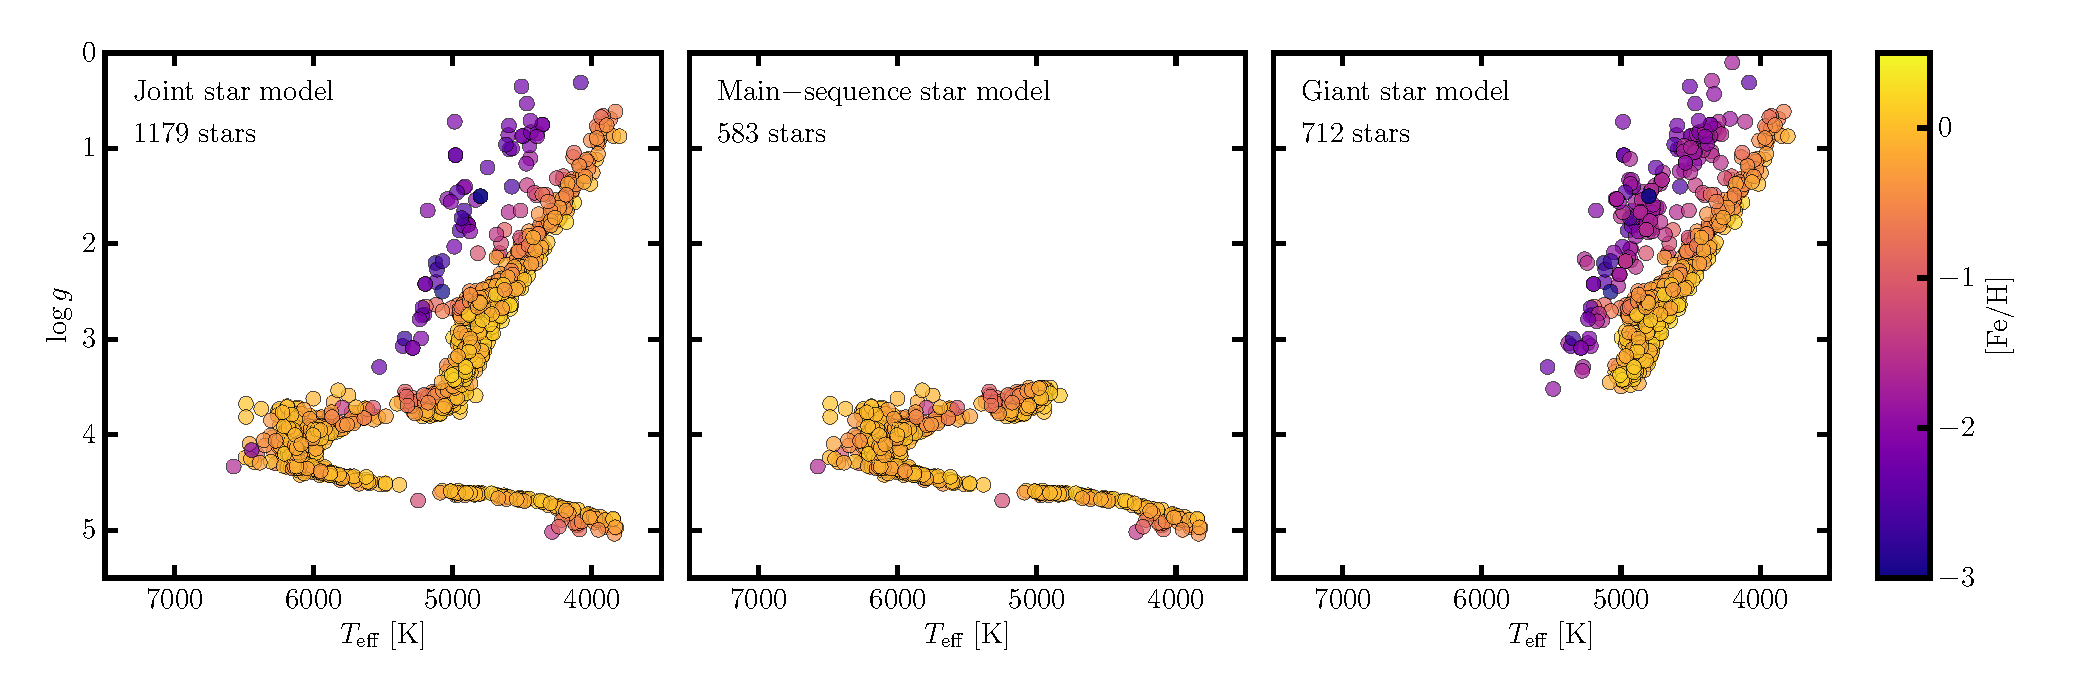
\includegraphics[width=\textwidth]{figures/hrd-train-set.pdf}
\caption{Effective temperature $\teff$ and surface gravity $\logg$ for all stars in the training sets. Stars are colored by their metallicity [Fe/H], and the three panels show stars in the joint model (left panel; Section~\ref{sec:a-simple-model}), the main-sequence star model (middle panel; Section~\ref{sec:unevolved-star-model}), and the giant star model (right panel; Section~\ref{sec:evolved-star-model}).\label{fig:training-set-hrd}}
\end{figure}


\begin{figure*}[p]
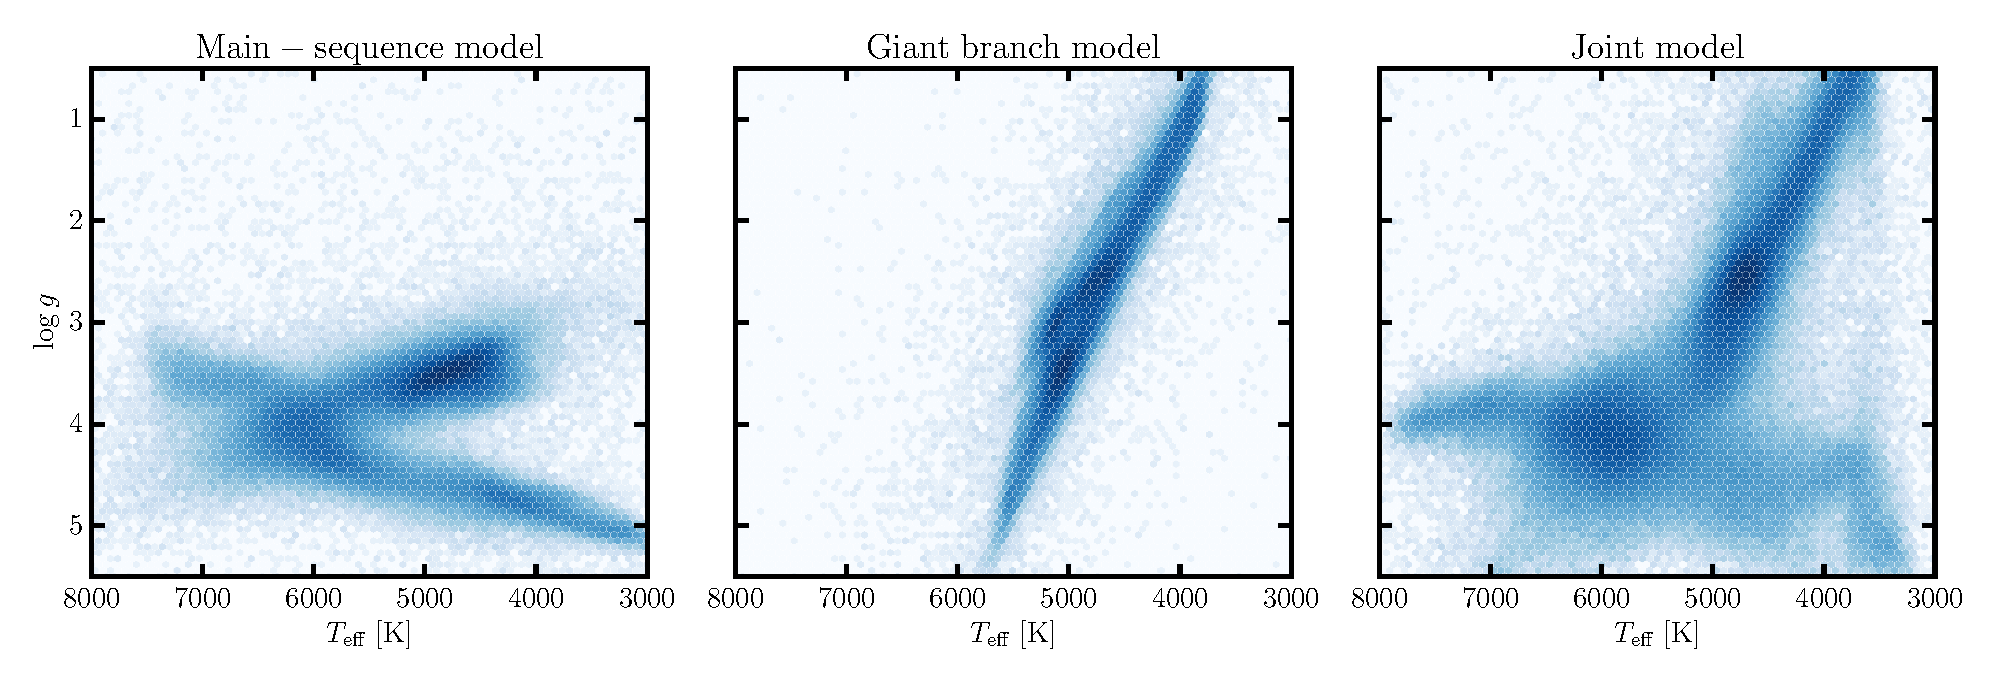
\includegraphics[width=\textwidth]{figures/test-set-density.pdf}
\caption{The logarithmic density of effective temperature $\teff$ and surface gravity $\logg$ for all \Nspectra\ \rave\ spectra, as derived using the joint model (left panel; Section~\ref{sec:a-simple-model}), the main-sequence star model (center panel; Section~\ref{sec:unevolved-star-model}), and the giant star model (right panel; Section~\ref{sec:evolved-star-model}). These panels demonstrate how a single quadratic model is insufficient for all \rave\ stars (left panel), and illustrate some of the systematic artefacts that can result from testing on stars outside of the training set (center and right panel).  These panels do not represent our final results, which are shown in Figure~\ref{fig:test-set-hrd}.\label{fig:test-set-density}}
\end{figure*}


\begin{figure}[p]
\center
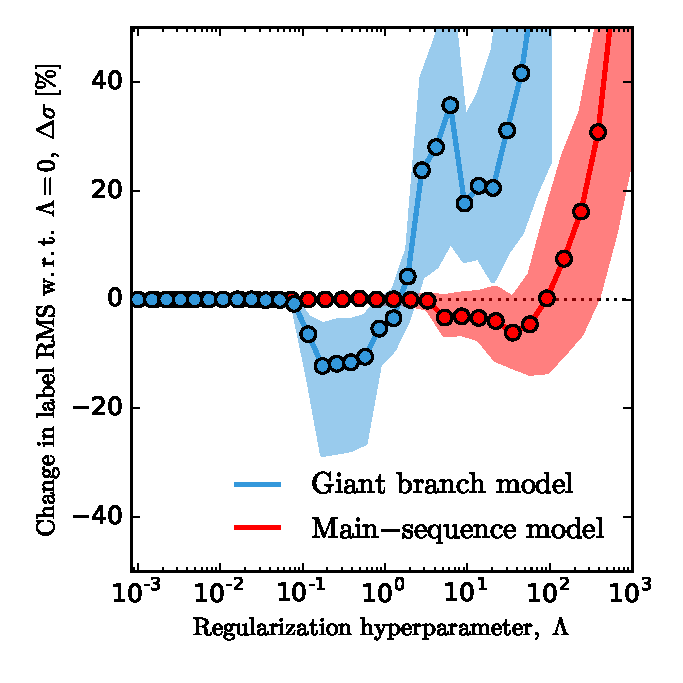
\includegraphics[width=0.45\textwidth]{figures/set-hyperparameters.pdf}
\caption{The percentage change in RMS deviation between inferred and training labels at different regularization strengths.  The RMS values were calculated by leave-one-out cross-validation, and are shown with respect to an unregularized model ($\Lambda = 0$).  The points and solid line indicate the mean improvement across all labels. The filled area represents the minimum and maximum improvements over all labels. With increasing regularization strength, there is a minimum in the RMS deviation over all labels, which is where we set $\Lambda$ for each model (see text for details).\label{fig:set-hyperparameters}}
\end{figure}


\begin{figure}[p]
\center
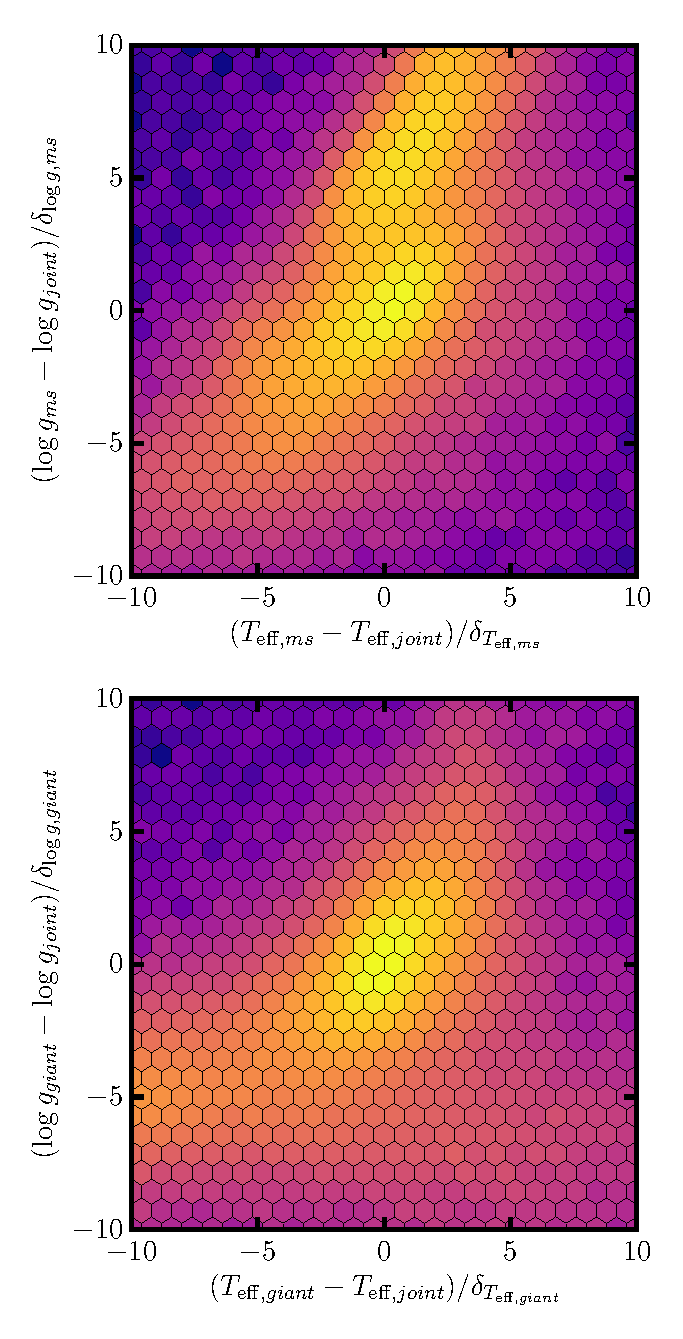
\includegraphics[width=0.5\textwidth]{figures/joint-model-differences.pdf}
\caption{The normalized differences in effective temperature $\teff$ and surface gravity $\logg$ between the main-sequence model and the joint model (top panel), and the giant model and the joint model (bottom panel).  The density scaling is logarithmic, and the differences in $\teff$ and $\logg$ are scaled to make them approximately isotropic (see text for details).  The peak at $(0, 0)$ represents good agreement between the joint model and comparison model, whereas the over-densities elsewhere are a consequence of testing the model on stars very different to the training set (e.g., dwarf stars tested on a model trained with only giant stars).\label{fig:joint-model-differences}}
\end{figure}


\begin{figure}[p]
\center
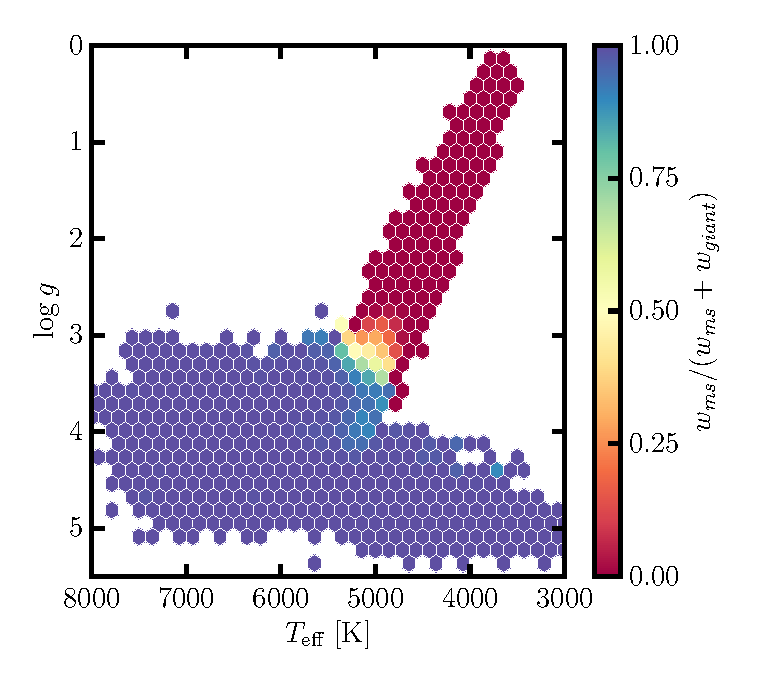
\includegraphics[width=0.5\textwidth]{figures/model-weights.pdf}
\caption{The mean relative main-sequence model weight $w_{ms}/(w_{ms} + w_{giant})$ at each hexagonal bin of weighted effective temperature $\teff$ and surface gravity $\logg$.  The relative weighting illustrates how only results from the main-sequence model are adopted for unevolved stars, and there is a gradual transition to using results from the giant model, before only results from the giant model are used for evolved stars.\label{fig:model-weights}}
\end{figure}


\begin{figure}[p]
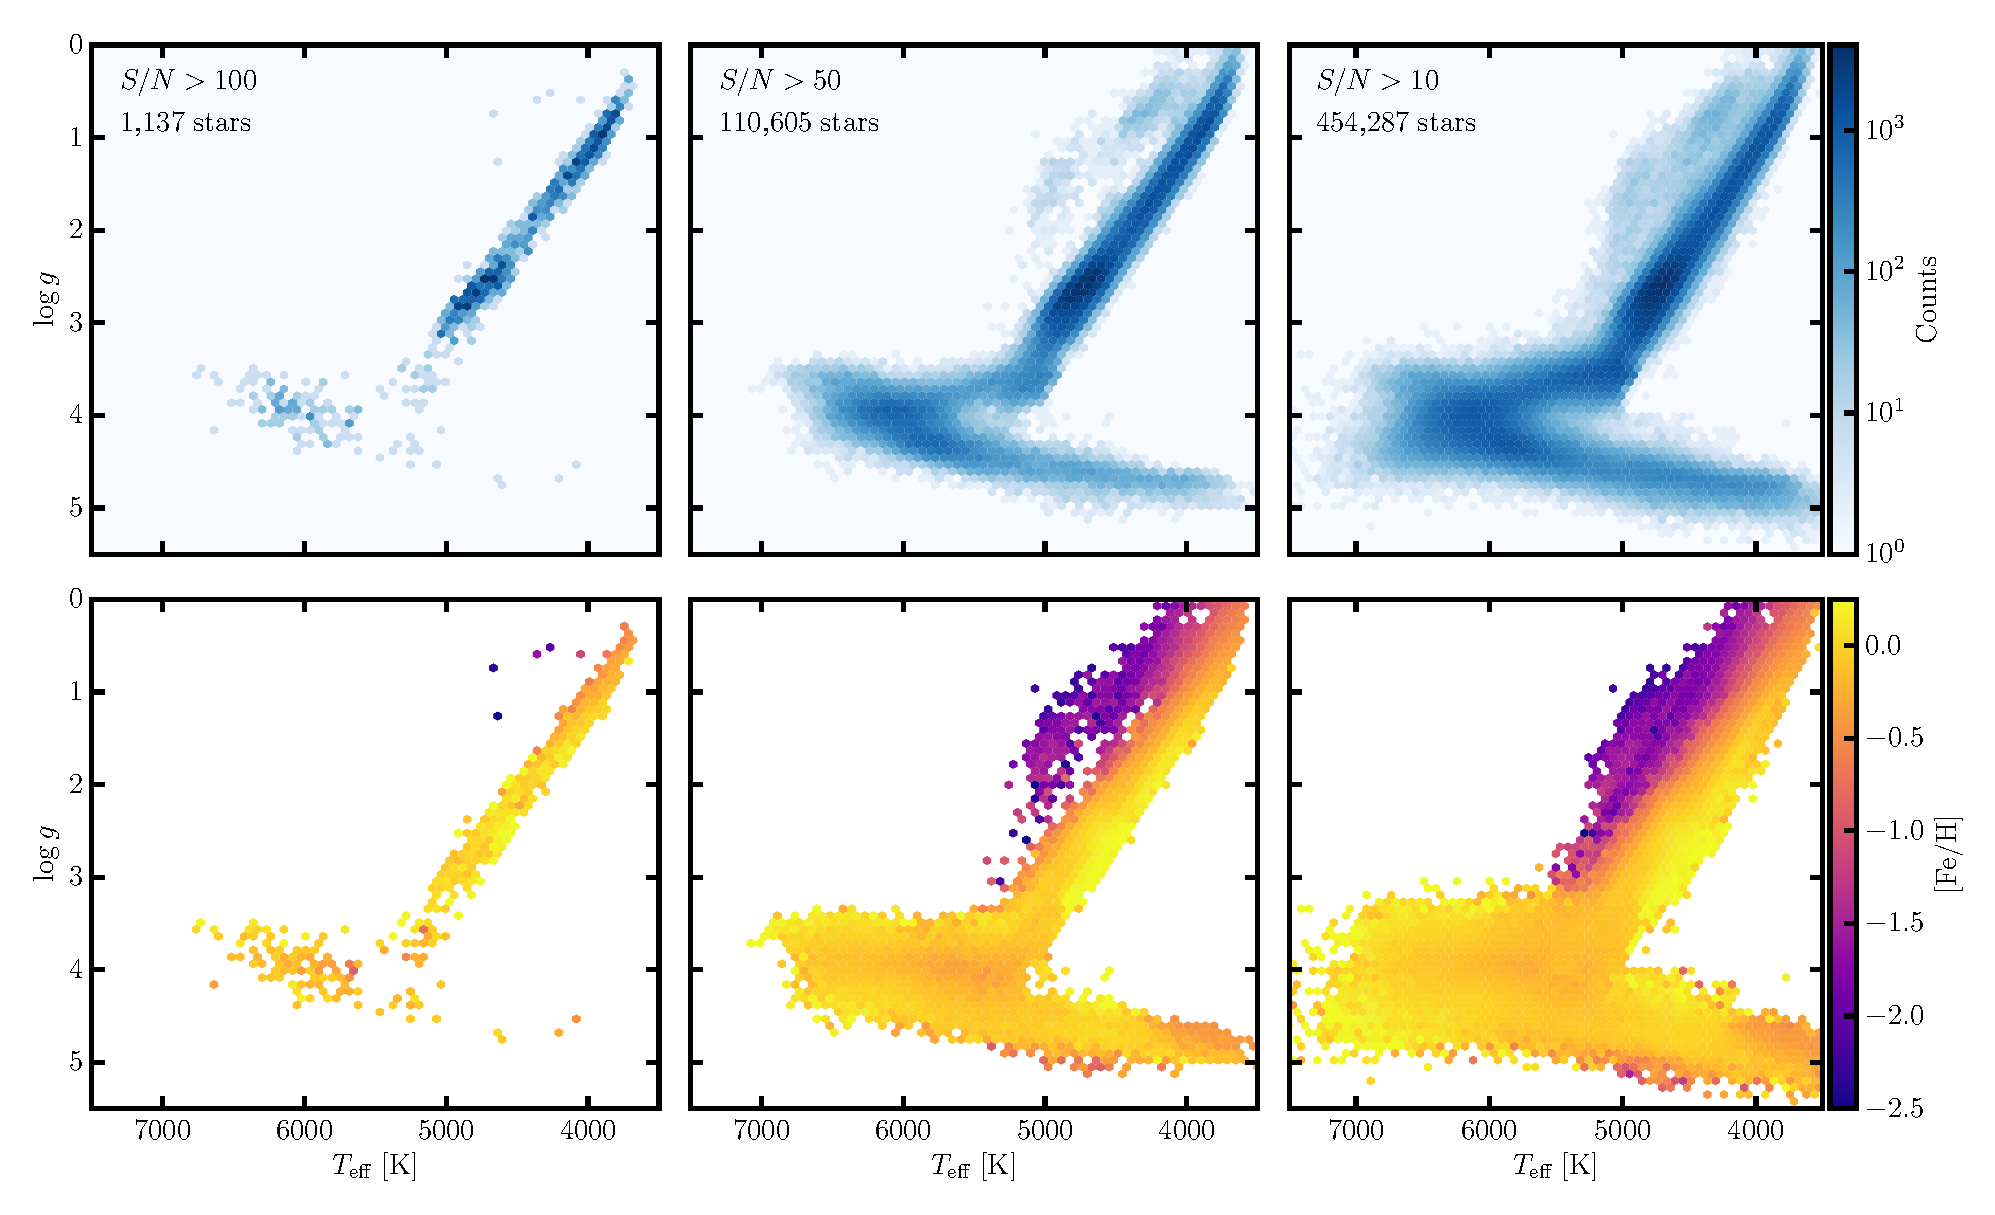
\includegraphics[width=\textwidth]{figures/hrd-test-set.pdf}
\caption{The effective temperature $\teff$ and surface gravity $\logg$ for \rave\ stars after combining labels from the main-sequence and giant star models.  Only results with $\chi_{r}^2 < 3$ and S/N ratios greater than the quoted limit in each panel are shown.  The top three panels show logarithmic density, and bins in the bottom three panels are colored by the median metallicity in each bin.\label{fig:test-set-hrd}}
\end{figure}


\begin{figure*}[p]
\caption{Distribution of differences in label estimates from multiple visits, divided by their formal errors summed in quadrature.  If our measurements were unbiased and the formal errors were representative, these distribution should be normally distributed with zero mean and unit variance.\label{fig:formal-errors-comparison}}
\end{figure*}


\begin{figure*}[p]
\caption{The RMS of the test set labels as a function of S/N ratio for repeated stars in the test set.\label{fig:test-set-repeats}}
\end{figure*}


\begin{figure*}[p]
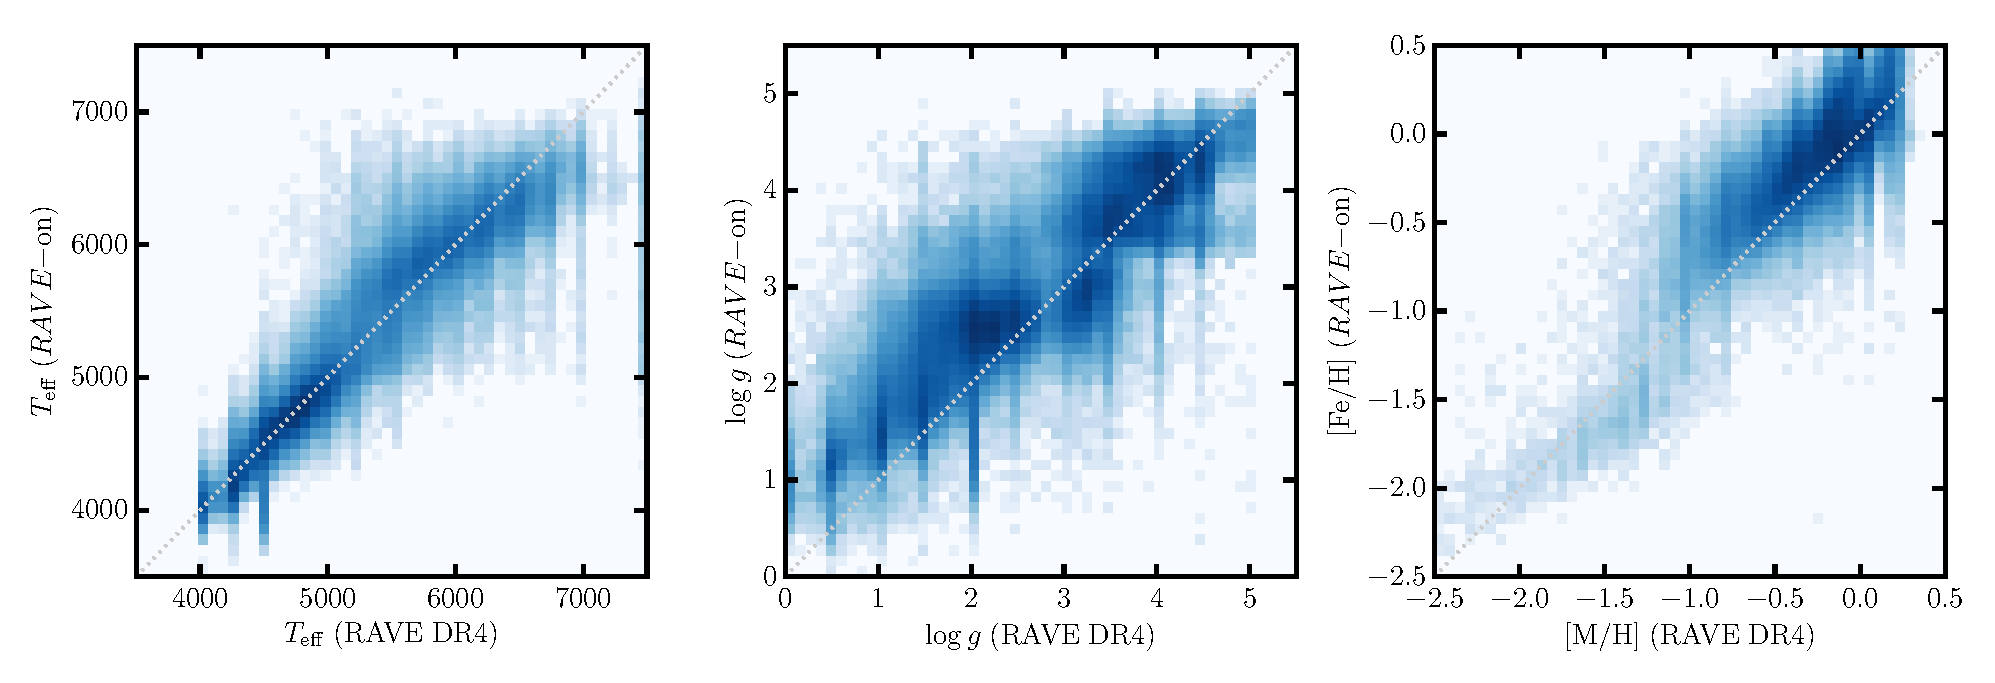
\includegraphics[width=\textwidth]{figures/dr4-comparison.pdf}
\caption{Stellar parameter ($\teff$, $\logg$, [Fe/H]) comparison between the fourth \rave\ data release \citep{Kordopatis_2013} and this work. Here we show the `calibrated' metallicity (column \texttt{c\_M\_H\_K}) from the \rave\ survey. Only stars meeting quality constraints in \emph{both} studies are shown (see text for details).\label{fig:rave-dr4-comparison}}
\end{figure*}


\begin{figure*}[p]
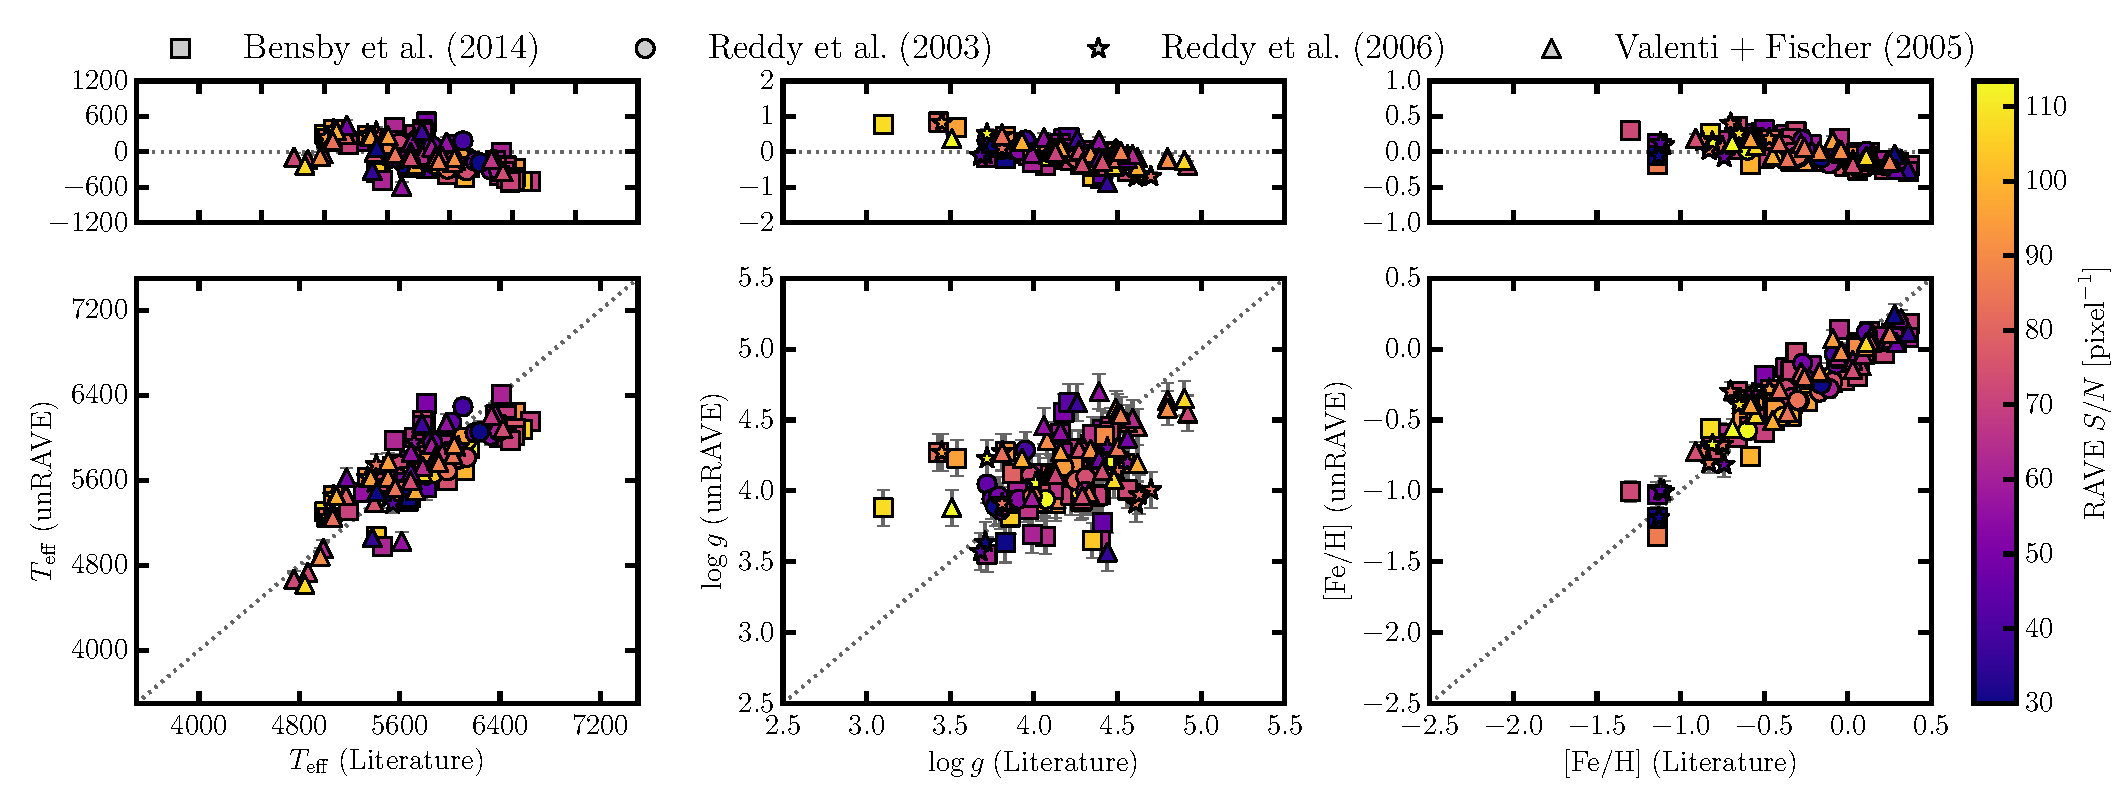
\includegraphics[width=\textwidth]{figures/gold-standard-comparison.pdf}
\caption{Stellar parameter ($\teff$, $\logg$, [Fe/H]) comparisons for stars in common between this work and `gold standard' studies that use high-resolution, high S/N spectra and \hipparcos\ parallaxes where available: \citet{Bensby_2014,Reddy_2003,Reddy_2006,Valenti_Fischer_2005}. Stars are colored by the S/N of the \rave\ spectra, and only stars with $\chi_r^2 < 3$ and S/N $> 10$ are shown.  \label{fig:gold-standard-comparison}}
\end{figure*}


\begin{figure*}[p]
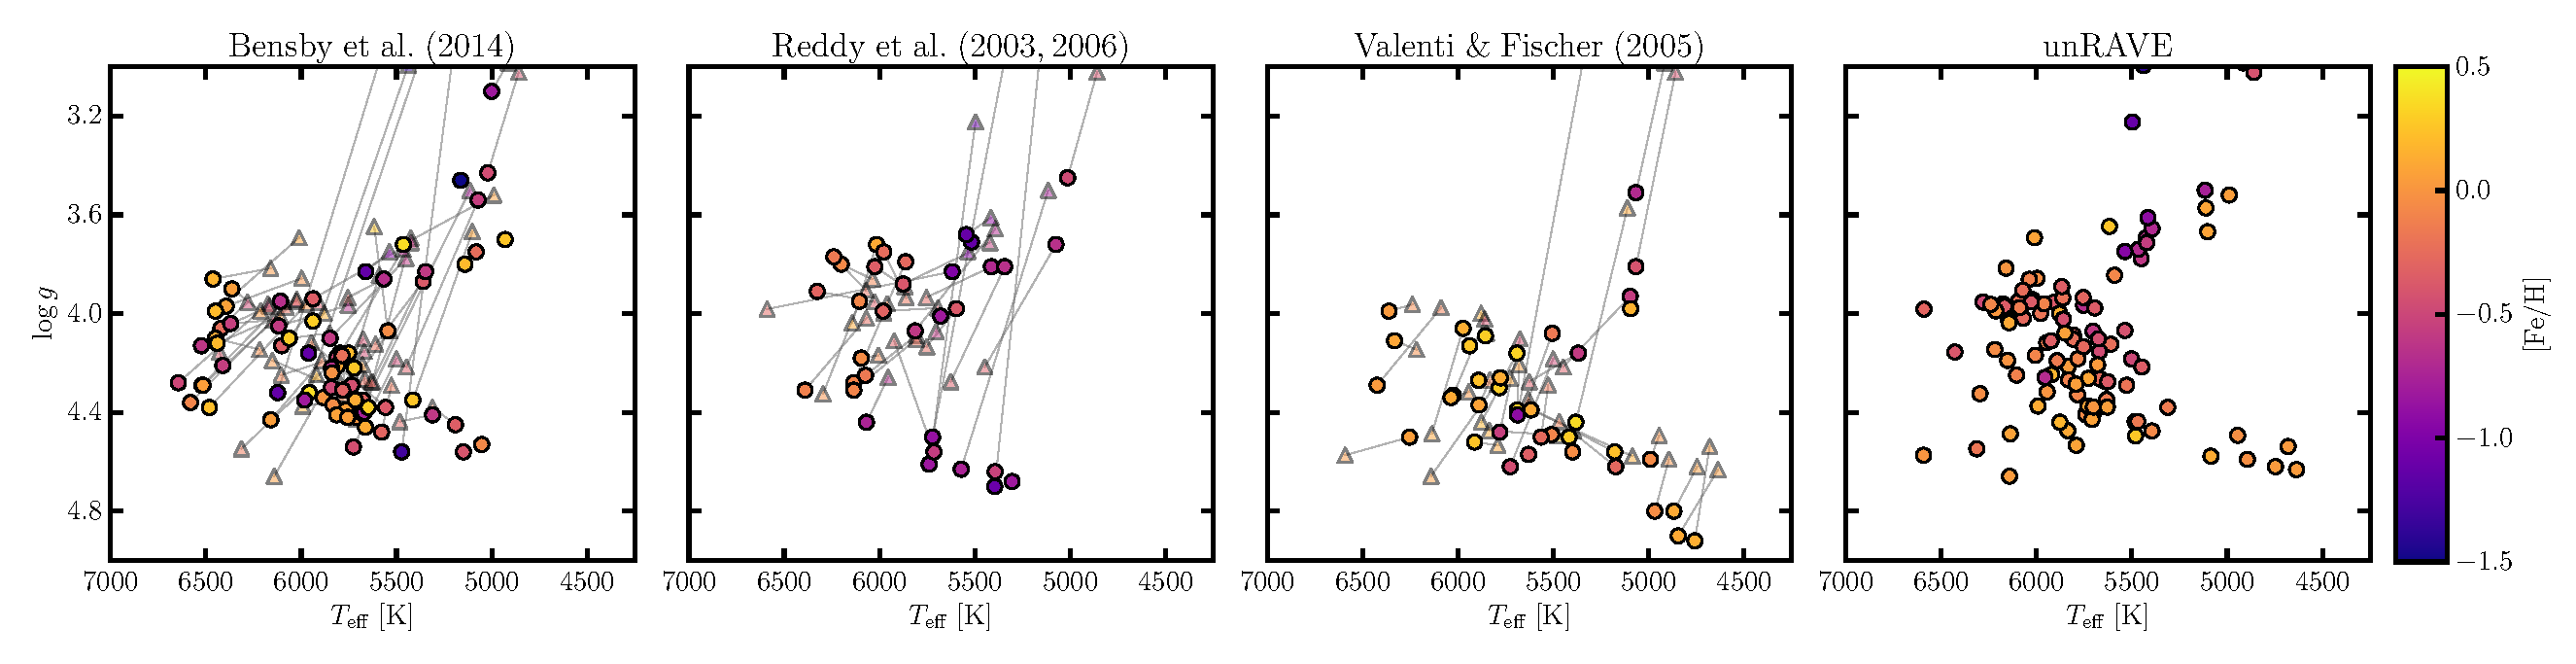
\includegraphics[width=\textwidth]{figures/gold-standard-hrd.pdf}
\caption{Hertsprung-Russell diagrams of stars in common between this work and that of \citet{Bensby_2014,Reddy_2003,Reddy_2006,Valenti_Fischer_2005}.  Stars are colored by the metallicity of each study. Circles indicate literature markers in the first three panels, and the linked triangles indicate \project{unRAVE} parameters for the same object. This figure illustrates the good overall agreement in the shape of the turnoff and sub-giant branch, yet also demonstrates how some literature metal-poor ($[{\rm Fe/H}] \lesssim -1$) dwarfs near the turn-off appear as metal-poor sub-giants in \project{unRAVE}.\label{fig:gold-standard-hrd}}
\end{figure*}


\begin{figure*}[p]
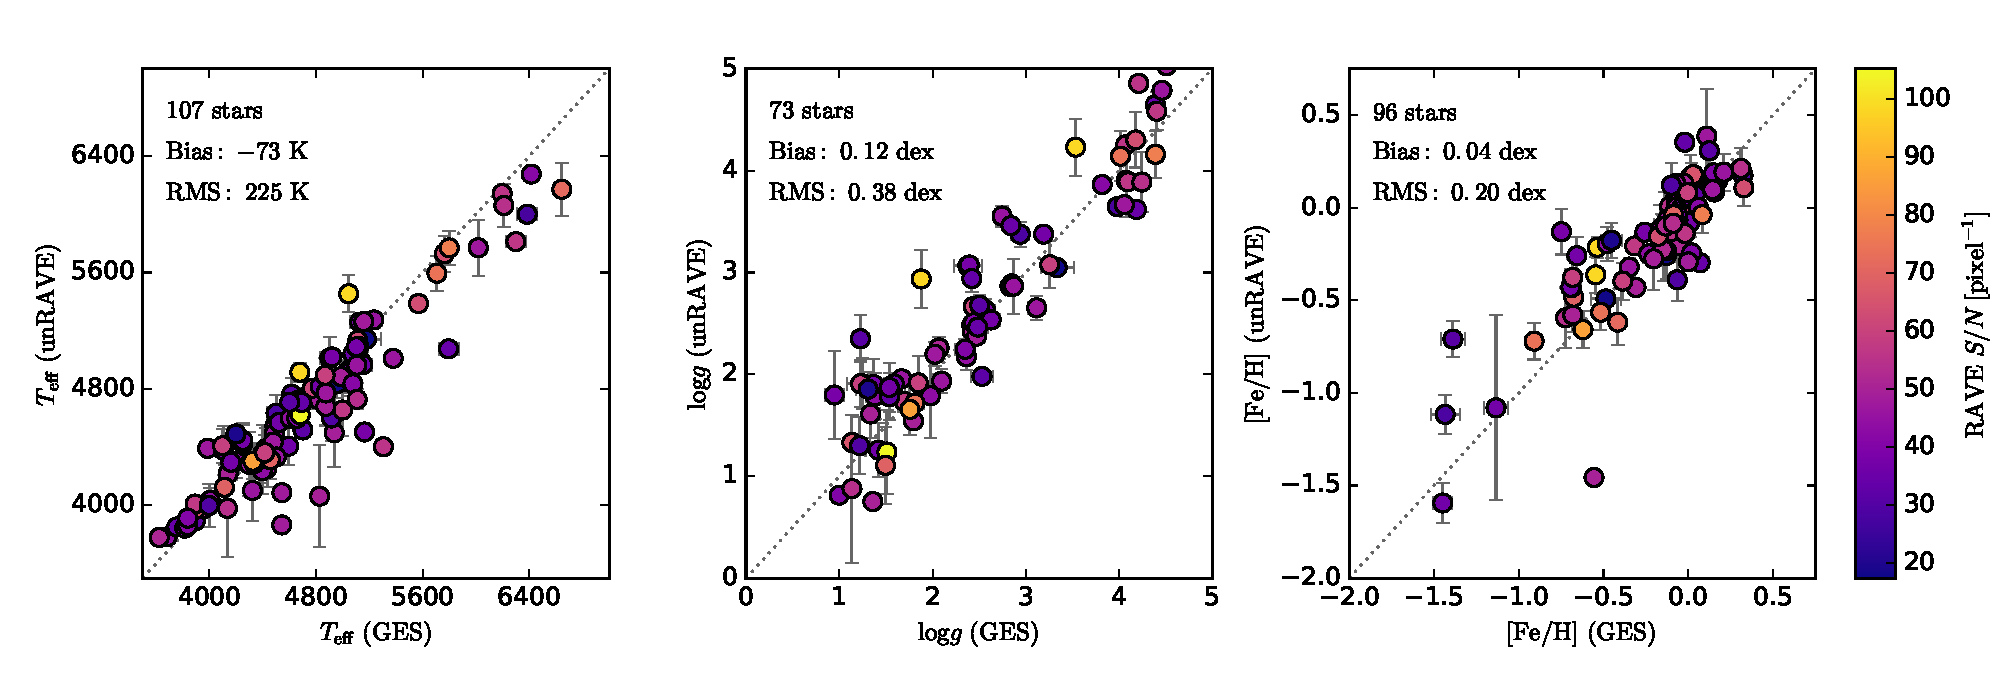
\includegraphics[width=\textwidth]{figures/ges-comparison.pdf}
\caption{Stellar parameter ($\teff$, $\logg$, [Fe/H]) comparison between the fourth internal data release from the \ges\ survey, and this work. The number of stars in each panel are shown, as well as the bias and RMS deviation in each label. Stars are colored by the S/N of the \rave\ spectra, and only stars with $\chi_r^2 < 3$ and S/N $> 10$ are shown.  Most of the \ges/\rave\ overlap stars have relatively low S/N ratios in \rave, near $\approx 30$~pixel$^{-1}$.\label{fig:ges-stellar-parameters}}
\end{figure*}


\begin{figure*}[p]
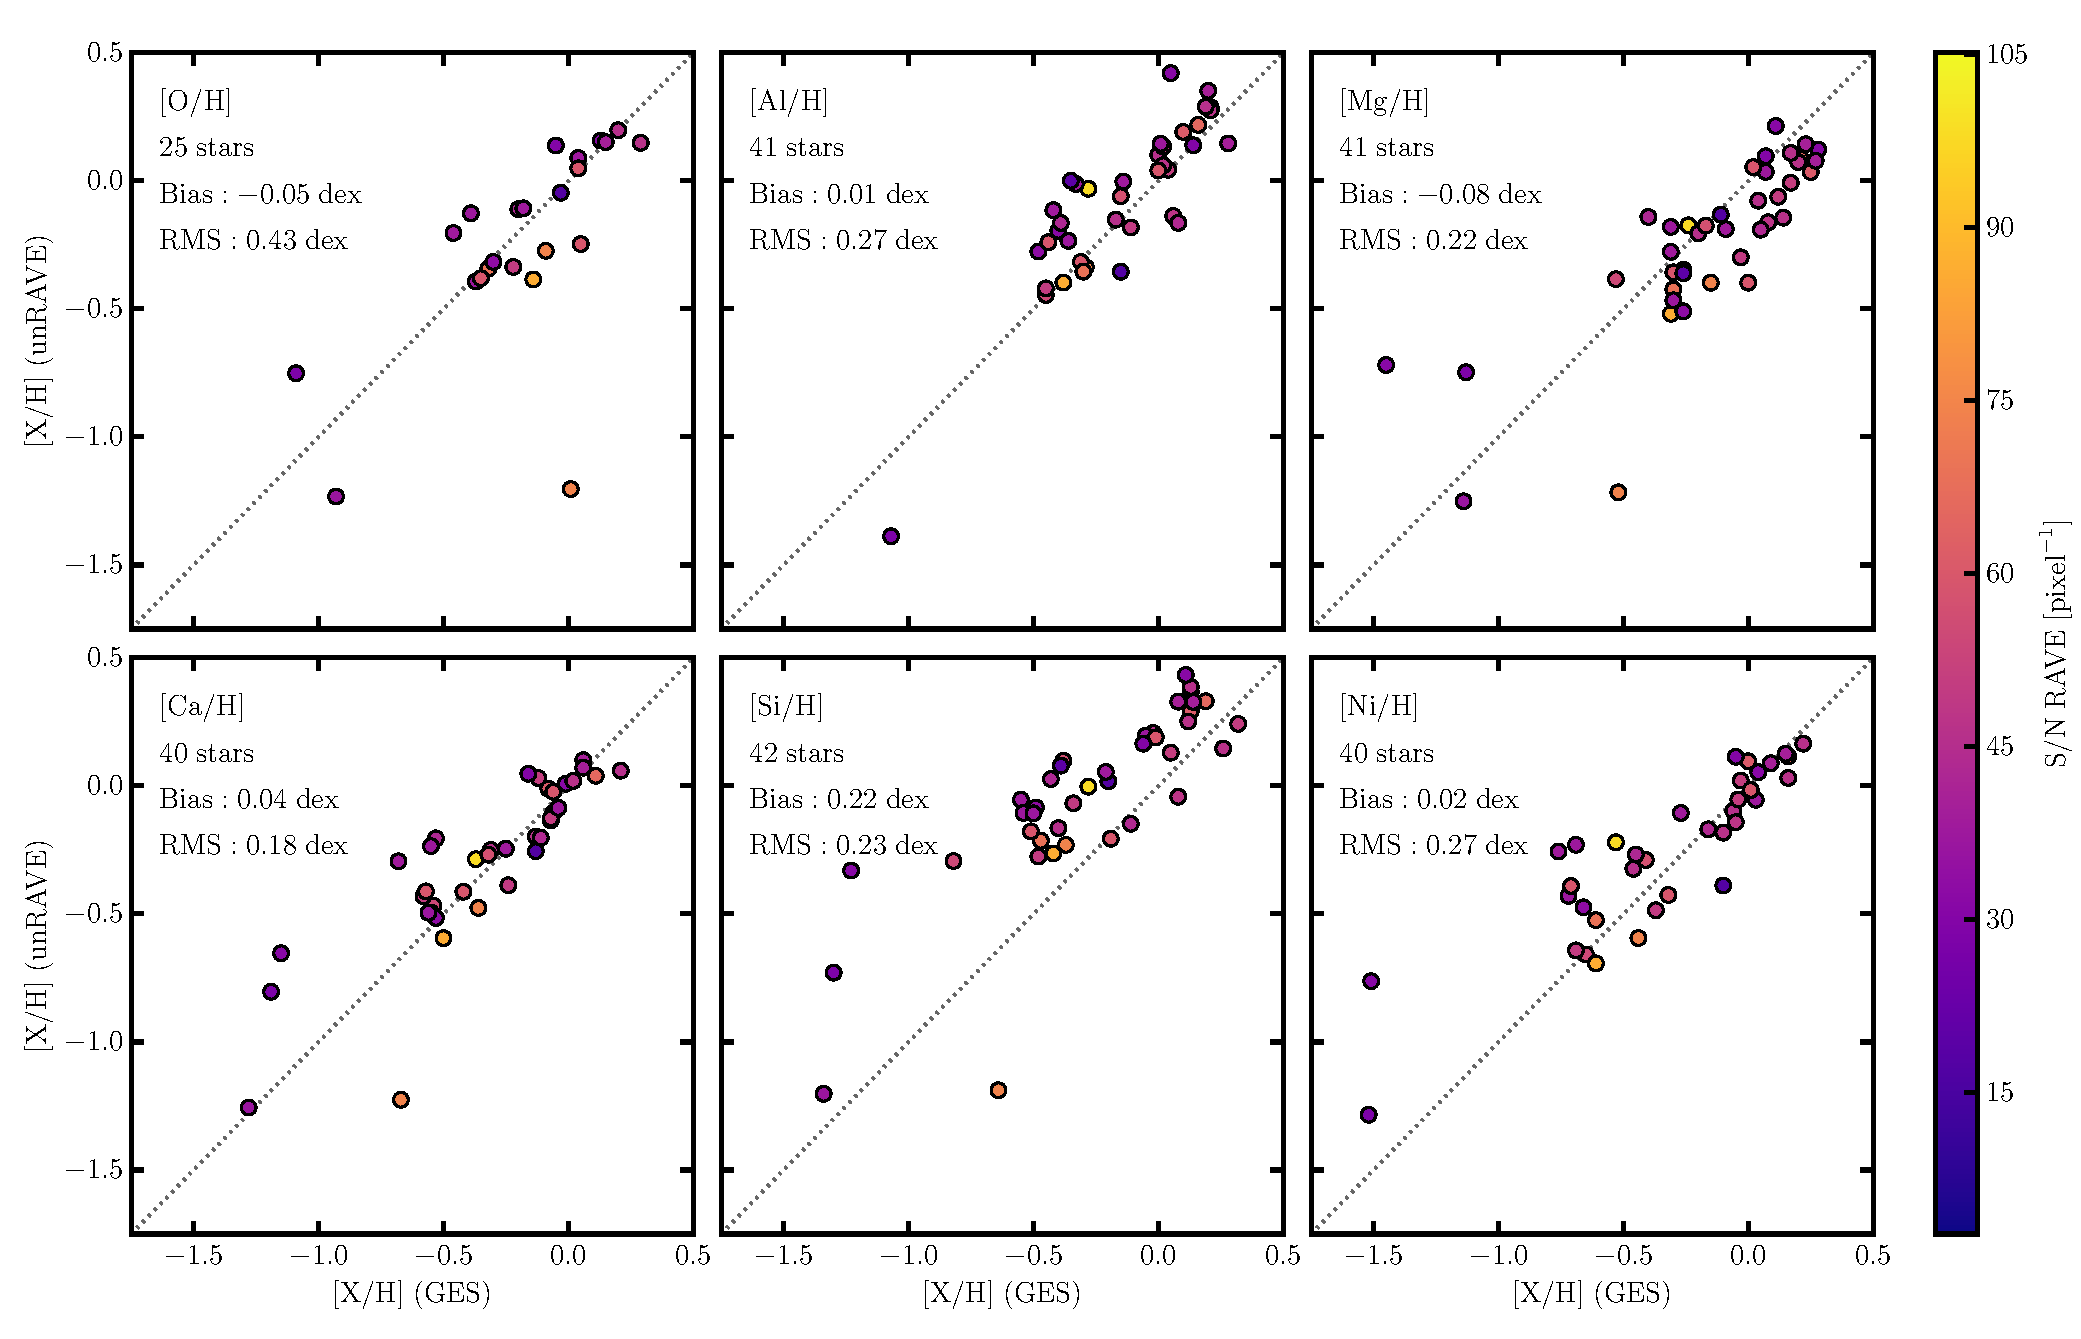
\includegraphics[width=\textwidth]{figures/ges-abundances.pdf}
\caption{Detailed chemical abundances in the fourth internal data release from the \ges\ survey compared to this work.  The number of stars shown in each panel is indicated, and the bias and RMS deviations are shown. Stars are colored by the S/N of the \rave\ spectra, and only stars with $\chi_r^2 < 3$ and S/N $> 10$ are shown.\label{fig:ges-abundances}}
\end{figure*}


\begin{figure*}[p]
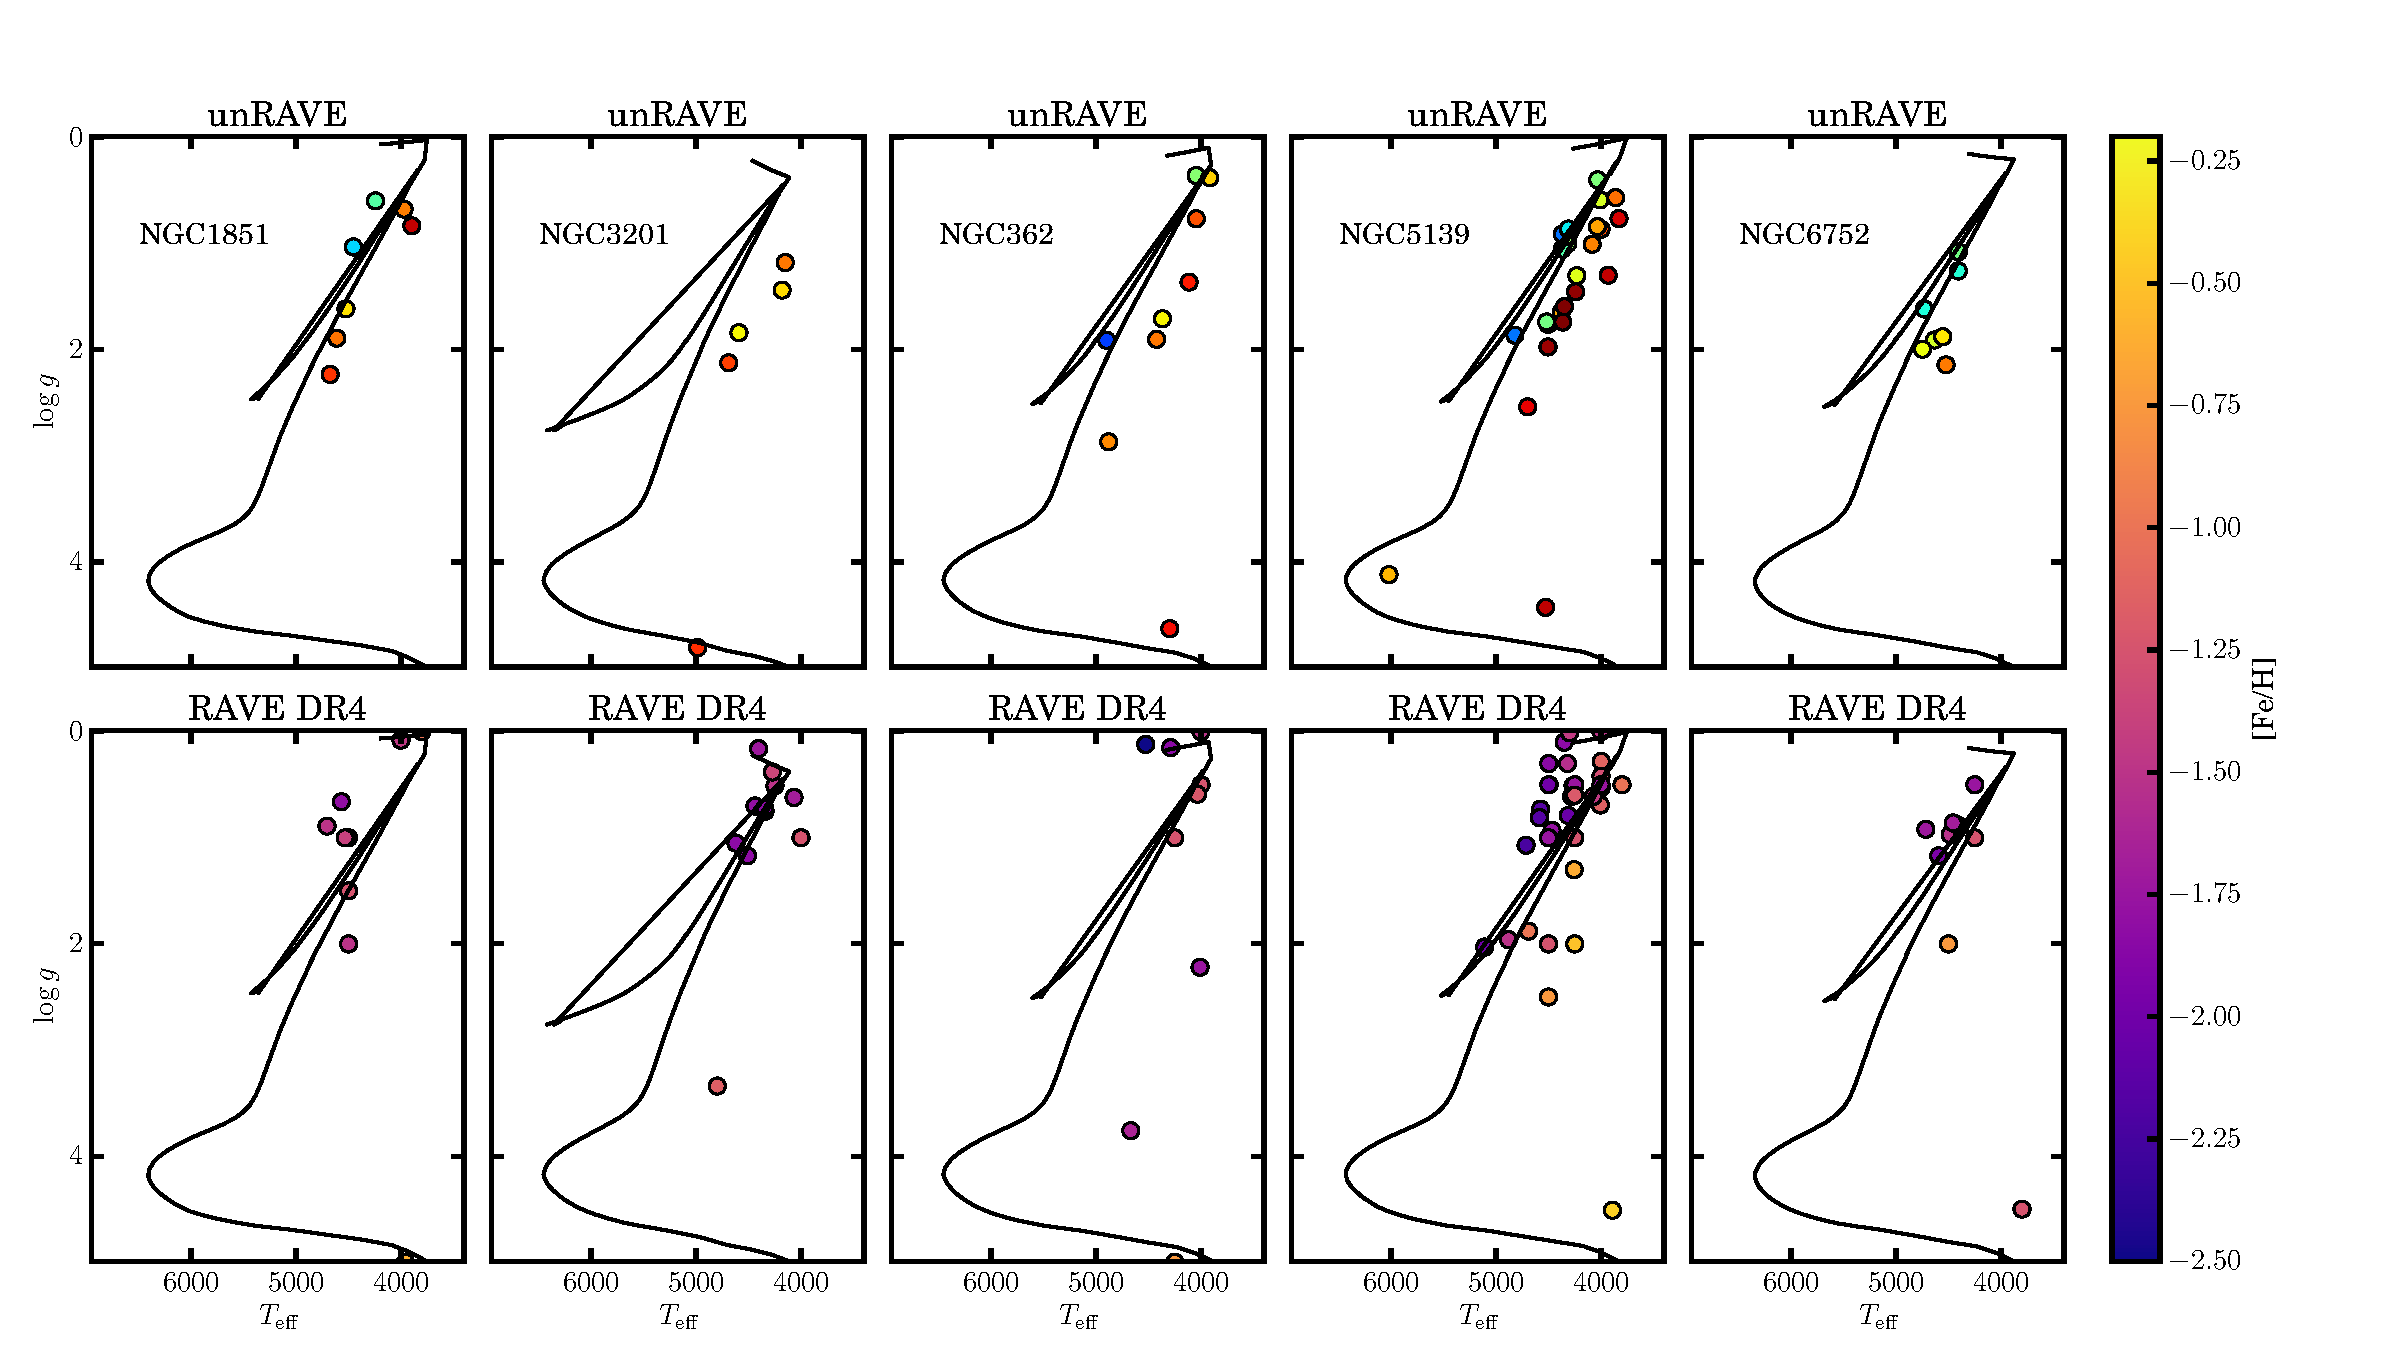
\includegraphics[width=\textwidth]{figures/HRD_GCs.pdf}
\caption{Top panels: Effective temperature $\teff$ and surface gravity $\logg$ from this work for prescribed members of globular clusters from \citet{Anguino_2014,Kunder_2014}. Bottom Panels: The same stars are shown as per the top panels, where $\teff$ and $\logg$ have been sourced from the fourth \rave\ data release. A representative Padova \citep{Bressan_2012} isochrone is shown for each cluster in each panel.
\label{fig:globular-cluster-HRD}}
\end{figure*}


\begin{figure*}[p]
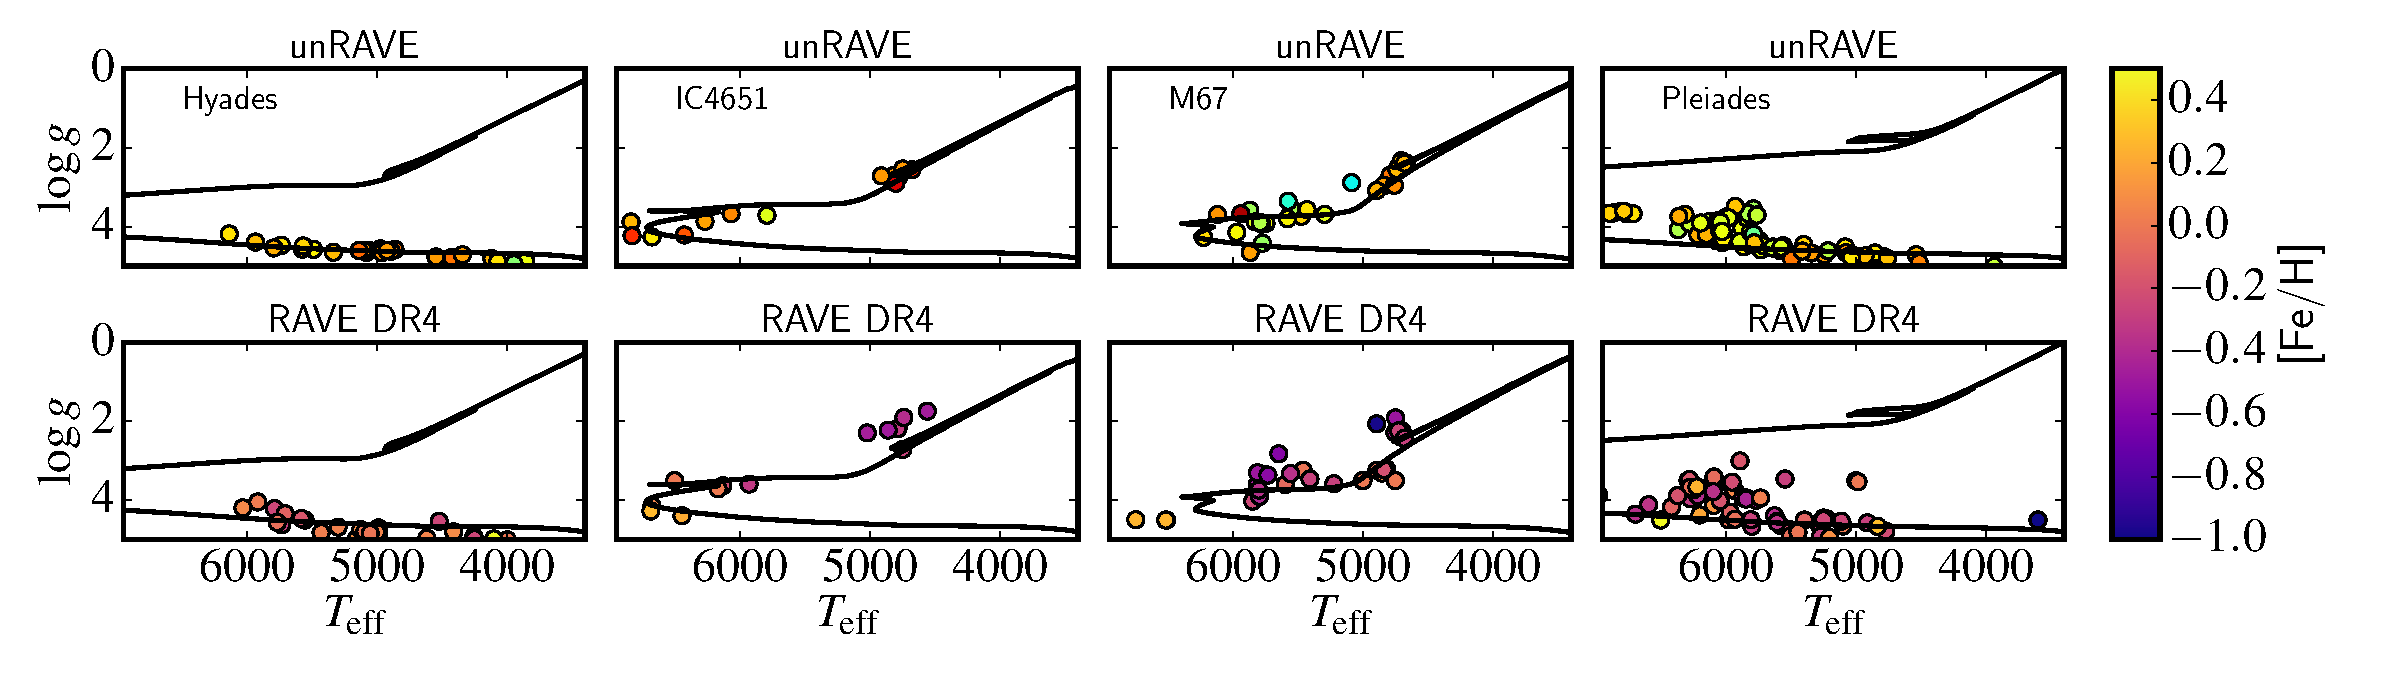
\includegraphics[width=\textwidth]{figures/HRD_OCs.pdf}
\caption{Top panels: Effective temperature $\teff$ and surface gravity $\logg$ from this work for prescribed members of open clusters from \citep{Kunder_2016}.  The same stars are shown for each open cluster in the bottom panels, where the $\teff$ and $\logg$ entries are sourced from the fourth \rave\ data release.\label{fig:open-cluster-HRD}}
\end{figure*}


\begin{figure*}[p]
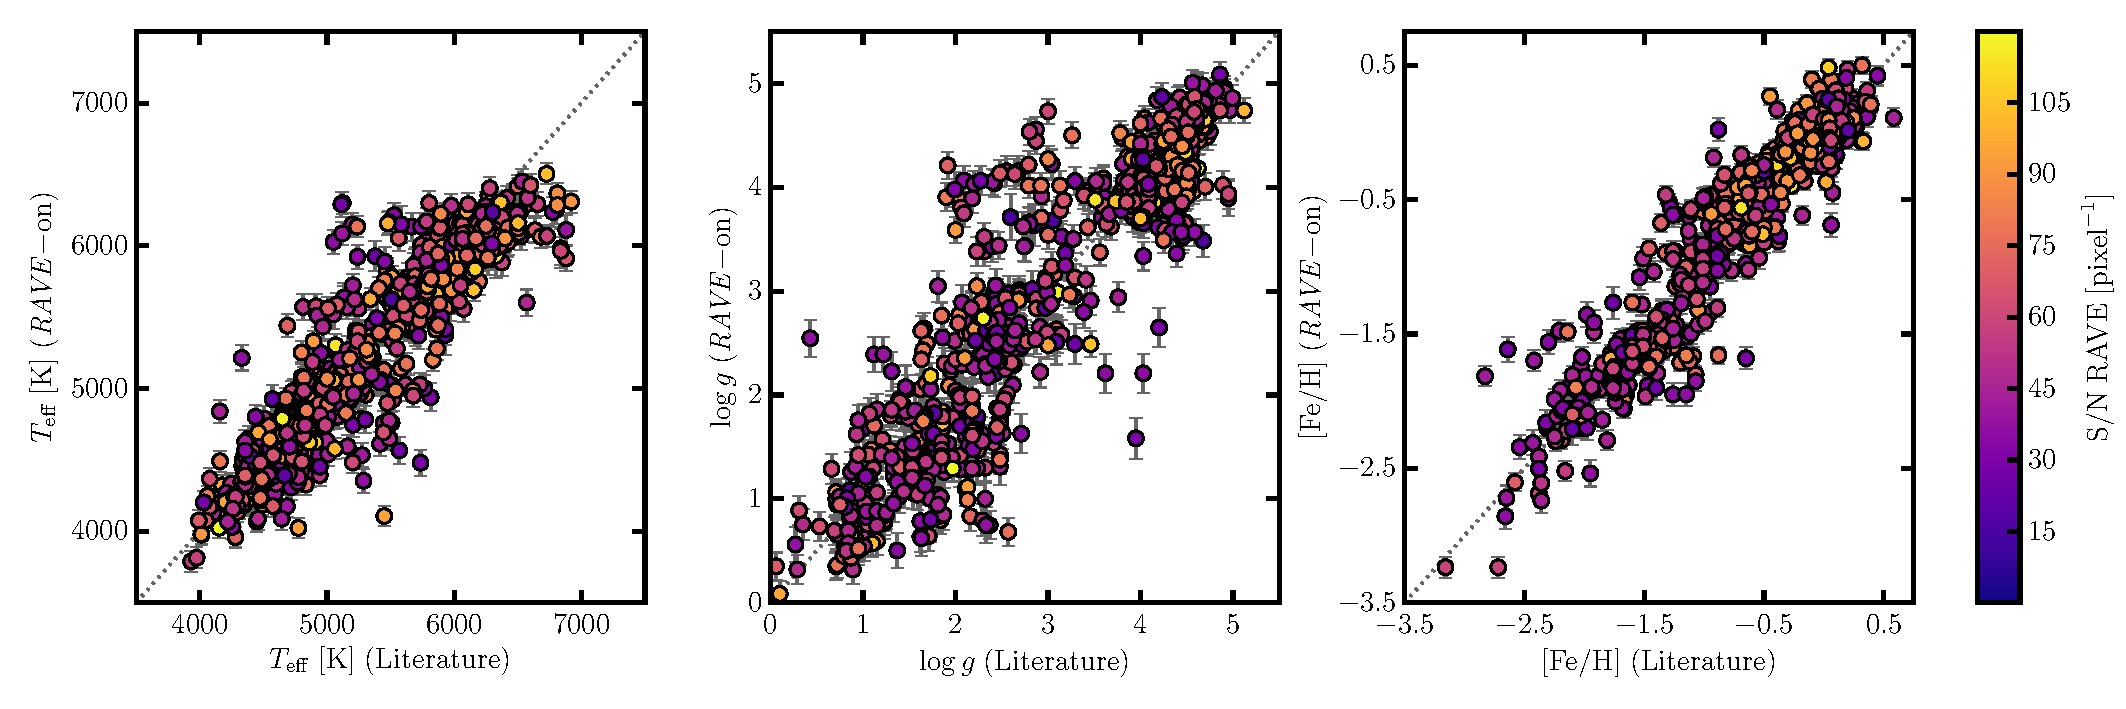
\includegraphics[width=\textwidth]{figures/kordopatis-calibration.pdf}
\caption{Stellar parameter ($\teff$, $\logg$, [Fe/H]) comparison with the literature calibration sources used by \citet{Kordopatis_2013} and \citet{Kunder_2016}. Stars are colored by the S/N of the \rave\ spectra. Note that this comparison is for illustrative purposes only: it is not an indication of independent agreement with the literature because some metal-poor stars in this literature sample were used in the construction of our training set (see text for details).\label{fig:kordopatis-calibration}}
\end{figure*}


\begin{figure}[p]
\center
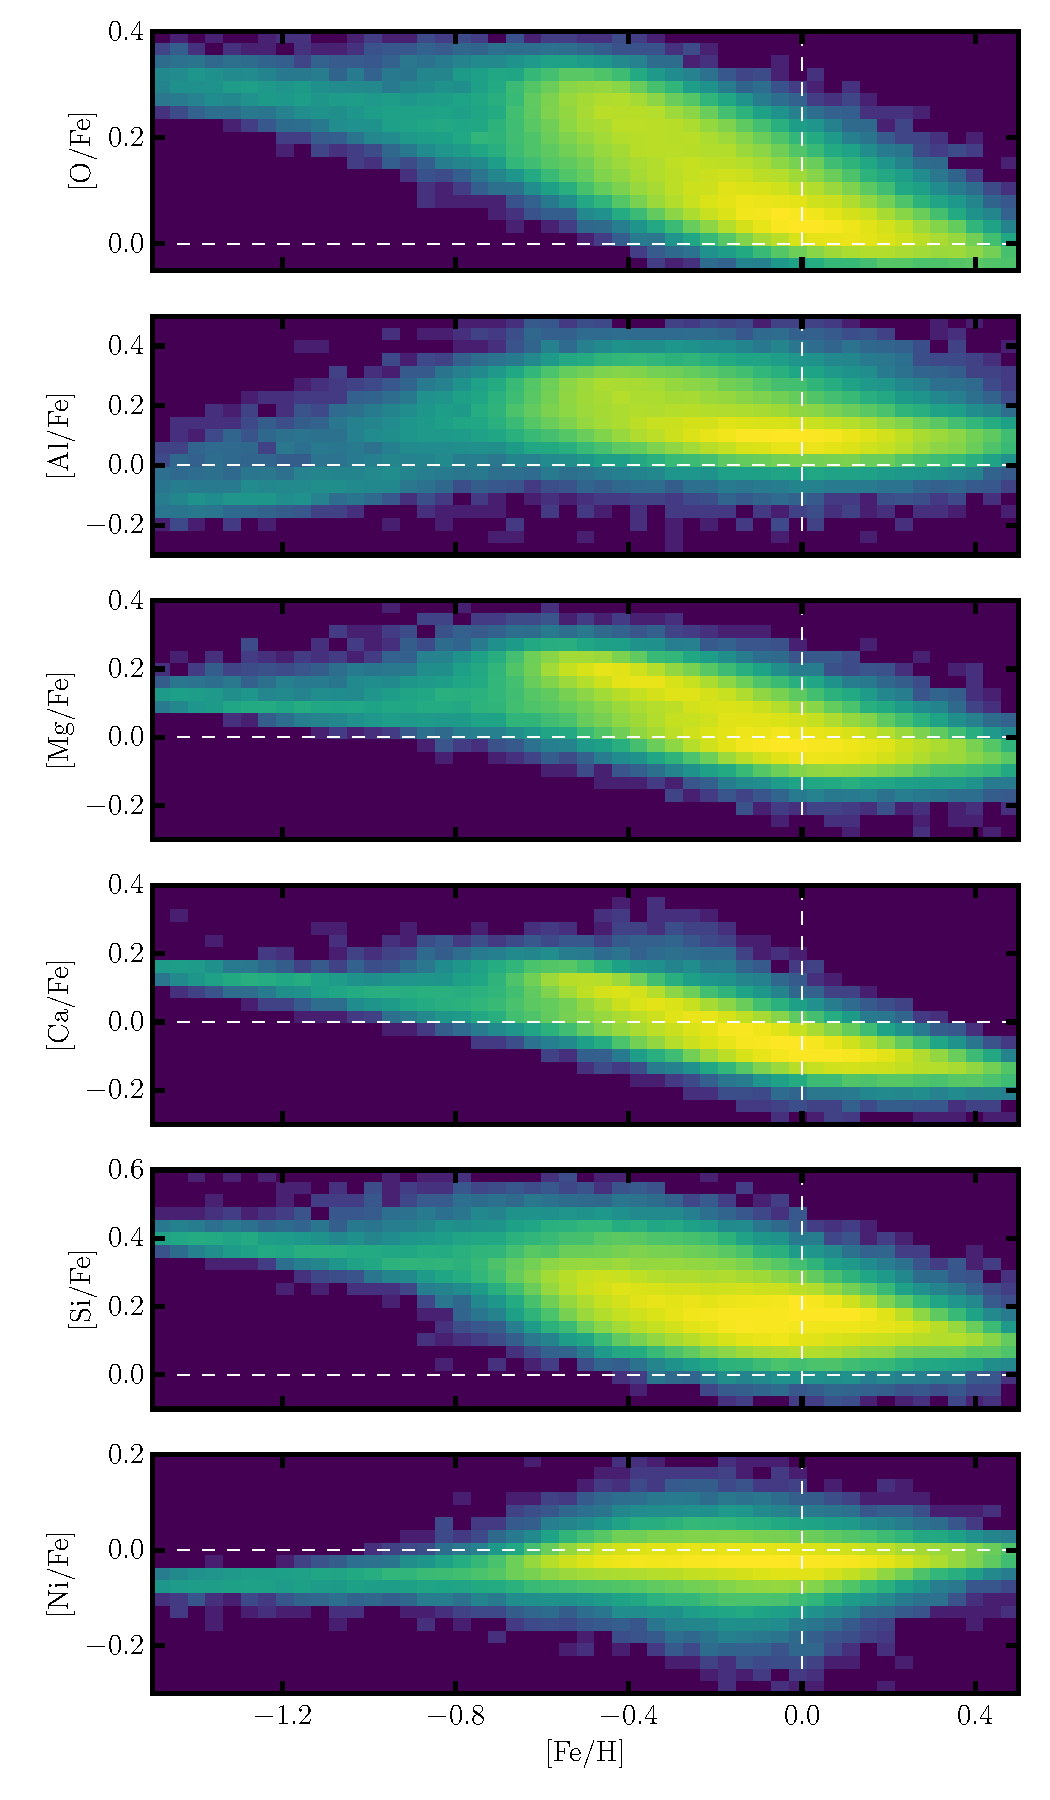
\includegraphics[width=0.65\textwidth]{figures/gce.pdf}
\caption{Detailed chemical abundances ([X/Fe]) for giant stars in \unrave\ with respect to [Fe/H], showing the Galactic chemical evolution derived for each element. Note that the y-axes limits vary for each panel, however for clarity we show the scaled-Solar position by dashed lines, and have common tick mark spacing on the y-axis for all panels. Only stars with S/N $> 10$ and $\chi_r^2 < 3$ are shown.\label{fig:gce}}
\end{figure}


\end{document}
